\documentclass[12pt]{report}
\usepackage[latin1]{inputenc}
\usepackage[paper=a4paper,dvips,top=3cm,left=3cm,right=3cm, foot=1cm,bottom=3cm]{geometry}
\usepackage{picinpar}
\usepackage{graphicx} %Graphics package for \includegraphics
\usepackage{caption}
\usepackage{subcaption}
\usepackage{wrapfig} %Enables wrapping of text around figures and tables
\usepackage{subfig}
\usepackage{enumerate}
\usepackage{multirow}
\usepackage{SIunits}%SI unit symbol package
\usepackage{amsmath}
\usepackage{array, calc}
\usepackage{tabularx}
\usepackage{setspace}
\usepackage{verbatim} %Enables \begin{comment}...
\usepackage{cite}
\usepackage{float}
\usepackage{mathtools}
\usepackage{threeparttable}
\usepackage{standalone}
\usepackage{booktabs, dcolumn}
\usepackage{placeins}
\usepackage{fancyvrb}
\usepackage[printonlyused]{acronym}
\usepackage[titletoc]{appendix}

\numberwithin{figure}{section}

\tolerance = 5000 % LaTeX er normalt streng n�r det gjelder linjebrytingen.
\hbadness = \tolerance % Vi vil v�re litt mildere, s�rlig fordi norsk har s�
\pretolerance = 2000 % mange lange sammensatte ord.


\usepackage{afterpage}
\newcommand\blankpage{%
    \null
    \thispagestyle{empty}%
    \addtocounter{page}{-1}%
    \newpage}


%\newenvironment{packed_enum}{
%\newenvironment{enumerate}{
%\begin{enumerate}
  \setlength{\itemsep}{10cm}
  \setlength{\parskip}{18pt}
  \setlength{\parsep}{10pt}
%}{\end{enumerate}}


% \usepackage{nomencl}
% \makenomenclature
% \renewcommand{\nomname}{Abbreviations}


\providecommand{\e}[1]{\ensuremath{\times 10^{#1}}}

\usepackage{hyperref}

\begin{document}

%Forside
\thispagestyle{empty}
\begin{center}        
  \vspace{5mm}        
  \huge
  \textbf{RCU2 testing and design} \\
  \vspace{50mm}
  \Large
  {\bf{\textsl{Inge Nikolai Torsvik}}} \\
  %\textsl{Eksperimentalfysikk med prosjektoppgave} \\
  \vspace{20mm}
  %{\bf{\textsl{Oppgave 12}}} \\
  \vspace{5mm}
  %{\large \textsl {(Bachelor i Fysikk)}}\\
  \vspace{10mm}
  \centerline{\includegraphics[height=4cm,width=4cm]{uglo.png}}
  \Large
  \textsl{Master Thesis} \\
  \vspace{50mm}
  \large
  \textsl{Department of Physics and Technology} \\
  \textsl{University of Bergen} \\
  \vspace{10mm}
  \large
  \textsl{June 2014} \\

\end{center}

%\thispagestyle{empty}


\setcounter{page}{1}
\pagenumbering{Roman}

\section*{Abstract}

\newpage
\section*{Contents}
\tableofcontents
\newpage

\FloatBarrier
\section{Acronyms}
  \begin{acronym}[acronyms]
\acro{CERN}{European Council for Nuclear Research}
\acro{OCL}[OCL]{Oslo Cyclotron Laboratory}
\acro{UiB}[UiB]{University in Bergen}
\acro{DUT}[DUT]{Device Under Test}
\acro{UiO}[UiO]{University of Oslo}
\acro{RCU}[RCU]{Readout Control Unit}
\acro{RCU2}[RCU2]{Readout Control Unit 2}
\acro{ALICE}{A Large Ion Collider Experiment}
\acro{LHC}{Large Hadron Collider}
\acro{FEE}{Front End Electronic}
\acro{FEC}{Front End Card}
\acro{RAM}[RAM]{Random Access Memory}
\acro{FPGA}[FPGA]{Field Programmable Gate Array}
\acro{SEE}{Single Even Effect}
\acro{SEU}{Single Event Upset}
\acro{IC}{Integrated Circuit}
\acro{PCB}{Printed Circuit Board}
\acro{LVDS}{Low-Voltage Differential Signaling}
\acro{NI}{National Instruments}
\acro{DAQ}{data acquisition}
\acro{SPI}{Serial Peripheral Interface}
\acro{SF2}{SmartFusion2}
\acro{CML}{Current-Mode Logic}
\acro{TTC}{Timing, Trigger and Control}
\acro{LVPECL}{Low Voltage Positive Emitter Coupled Logic}
\acro{RAM}{Random access memory}
\acro{SRAM}{static RAM}
\acro{PM-tube}{PhotoMultiplier Tube}
\acro{TID}{Total Ionizing Dose}
\acro{JTAG}{Joint Test Action Group}
\acro{UART}{Universal Asynchronous Receiver/Transmitter}
\acro{VHDL}{VHSIC Hardware Description Language}
\acro{CHSIC}{Very High Scale Integrated Circuit}
\acro{CPU}{Central Processing Unit}
\acro{MCU}{Microcontroller Unit}
\acro{ADC}{Analog to Digital Converter}
\acro{LET}{Linear Energy Transfer}
\acro{SOC}{System On a Chip}



\end{acronym}
\FloatBarrier

\newpage
\setcounter{page}{1}
\pagenumbering{arabic}

\chapter{Introduction}
At \acf{CERN} in Switzerland there are being conducted experiment on fundamental structure of the universe. This is done by accelerating particles up to a energy of 4 $\tera \electronvolt$ per proton, and then crash with other particles with same energy. This experiment is done by connecting several accelerators with higher and higher energies together to accelerate particles. The last accelerator in the chain is called \acf{LHC}, and is the largest particle accelerator ever built, installed in a 27 $\kilo \meter$ long tunnel.
Particles are accelerated in both direction in the LHC. When the particles has reached high enough energy, particles from opposite direction are made to crash at 4 experiment areas, one of these is called \acf{ALICE}.
The \ac{ALICE} detector is built to study a matter known as Quark-gluons plasma \cite{ALICE}, which will be generated under collisions of heavy ions.
The detector consist of several sub-detector with different functionality. \ac{TPC} is one of these, and is the main tracking detector placed in the inner circle of \ac{ALICE}, see section \ref{ALICE_experiment}. Under a collision high energetic neutrons and protons will be generated, and will also pose a risk to the electronics used.
It is therefore of highest importance to test everything that are planed to be used in the experiment for radiation. A replacement of electronics after installed in the detector is normally impossible under a run period, which can last up to several years.
 
One of the main boards used in the \ac{TPC} detector is the \acf{RCU}. Now there has been decided that a new \ac{RCU} board shall be made, namely the \ac{RCU2}.
Everything that are going to be used in the \ac{LHC} tunnel has to be made sure that it can survive the radiation level that are there.
Therefore every \acf{IC} planned to be used for the design of the \ac{RCU2} board has to be tested for radiation to be sure that it won't fail when it is installed in the \ac{TPC} detector.

\section{How to test}
\label{how_to_test}
The radiation tests done through this thesis is mainly \ac{TID} test.
That is irradiation up to a level where an error can clearly be seen or when a high enough dose has been reached without detecting errors, see section \ref{TID} for more information.
But there has also been done tests for \ac{SEE}, like \acf{SEU}, \acf{SET} and \acf{SEL} on a Microsemi \ac{SF2} \ac{SoC} \ac{FPGA}.

\section{About this work}
When I started working with my thesis in the autumn of 2013 the schematic layout for the \ac{RCU2} was basically finished,
and most of the component was decided, but not all of the component had been tested.
My work through this thesis has been planing how to test different \ac{IC}, designing test setup and executing the tests.
For most of the \ac{IC} which has been tested throughout this thesis, a simple \ac{PCB} was made with only the necessary to make the \ac{IC} work and to be able to test it.
By the use of \acf{DAQ} boards from National Instruments, the \ac{PCB} was connected to a computer where inputs was controlled and the outputs and current consumption was measured through a labVIEW program. 
The \ac{RCU2} main \ac{FPGA} has also been tested. That is a Microsemi \ac{SF2} \ac{SoC} \ac{FPGA}. A \ac{SF2} starter-kit was used when designing test for this \ac{IC}, and test code was written in VHDL and C.
I also made a \ac{PCB} for measuring current and control a power regulator on the \ac{SF2} starter-kit.
The \acp{IC} which I have tested consist of: SoC FPGA, power regulators, bus transceivers, limiting amplifier, multiplexer/demultiplexer, buffer, comparator and Current Shunt Monitor.
Every \ac{IC} was irradiation tested in \ac{OCL} at the University of Oslo, the \ac{SF2} chip was also irradiation tested in \ac{TSL} in Uppsala in Sweden.

\newpage

\chapter{ALICE experiment}
\label{ALICE_experiment}
Since 1954 physicists at \ac{CERN} have studied the nucleus and its structure to find the fundamental structure of the universe.
\ac{CERN} is the world largest research center for nuclear and particle physics, and has a total of 21 member state.
One of the biggest and newest invention at \ac{CERN} is the \acf{LHC}, that is a circular particle accelerator placed in a 27 km long tunnel around 100 meter beneath ground level.
This is the last accelerator in a chain of up to 7 (depending on which particle to accelerate), see picture \ref{CERN_accelerators}, where the particles gradually accelerate to higher and higher energies, up to their maximum energy of 4 TeV and speed close to the s peed of light. When particles has reached this energy level accelerated particles from opposite direction are made to collide inside 4 different experiment areas, where one of these is called \acf{ALICE}. See figure \ref{ALICE_layout}.

The \ac{ALICE} detector is a heavy ion detector. Its main purpose is to study a state of matter called quark-qluon plasma\footnotemark which will be generated when heavy ions collides.
Under such a collision a temperature 100 000 times higher than the temperature of the sun is generated.
There is then high enough energy to split the protons and neutrons, and achieve a plasma of unbound quarks and gluons, and that is called quark-gluon plasma.

\footnotetext{All ordinary matter in today's universe is made up of atoms.
Each atom contains a nucleus composed of protons and neutrons (except hydrogen, which has no neutrons), surrounded by a cloud of electrons.
Protons and neutrons are in turn made of quarks bound together by other particles called gluons.
No quark has ever been observed in isolation: the quarks, as well as the gluons, seem to be bound permanently together and confined inside composite particles, such as protons and neutrons.
}

\begin{figure}[!htbp]
  \centering
  \includegraphics[width=0.65\textwidth]{CERN_accelerators.jpg}
  \caption{CERN accelerators \cite{website:CERN_accelerators}}
  \label{CERN_accelerators}
\end{figure}

\begin{figure}[!htbp]
  \centering
  \includegraphics[width=\textwidth]{ALICE_layout.jpg}
  \caption{Layout of the ALICE experiment \cite{website:aliceinfo}}
  \label{ALICE_layout}
\end{figure}

\FloatBarrier

\section{The Time Projection Chamber TPC}
The ALICE detector comprises of several sub-detectors, where one of these is the \acf{TPC}. \ac{TPC} is the main tracking detector placed in the inner circle of \ac{ALICE}.
The function of \ac{TPC} are tracking particles, measure the charged particles momentum and identification of particles.
A drawing of the \ac{TPC} can be seen in figure \ref{TPC_layout}.
The \ac{TPC} detector has a cylindrical shape, with a inner radius of 85 cm and outer radius of 250 cm, and has an overall length of 510 cm.
The detector is made up of a large cylindrical field cage, filled with 88 $m^3$ of 90\% Ne gas and 10\% $CO^2$ gas.
A high voltage electrode is placed in the center of the detector, dividing the \ac{TPC} into two drift regions, and making a electric field between electrode and the two end plates.
When a charged particle is generated inside the detector, the gas inside the cage will be ionized and make electrons drift in the electric field between the high voltage electrode and the two end plates.
At the end-plates we find the Readout Chamber which are divided into 18 trapezoidal sectors, where each sector is again divided into the inner and outer chamber.
In the readout chamber, there are a total of 560 000 readout pads of three different sizes: 4 $\times$ 7,5 $\milli\meter^2$ in
the inner chambers, 6 $\times$ 10 $\milli\meter^2$ and 6 $\times$ 15$\milli\meter^2$ in the outer chambers.

\begin{figure}[!htbp]
  \centering
  \includegraphics[width=\textwidth]{TPC_layout.png}
  \caption{Layout of the TPC \cite{website:aliceinfo}}
  \label{TPC_layout}
\end{figure}

\section{The TPC Front End electronics FEE}
Each of the total 36 sections (2 x 18) are also divided into 6 readout partitions, that is 2 in the inner chamber and 4 in the outer chamber. 
Each of the readout partitions are controlled by a \acf{RCU} which is connected to 18 to 25 \acf{FEC}. See figure \ref{TPC_Sections}
There are a total of 216 \ac{RCU} connected to a total of 4356 \ac{FEC} which is connected to all of the 560 000 readout pads, and all together this sums up the \acf{FEE}.
In short the task of the \ac{FEE} is to read out charge received at the readout pads, process it and send useful data to a computer.

\begin{figure}[!htbp]
  \centering
  \includegraphics[width=0.5\textwidth]{TPC_Sections.png}
  \caption{A TPC sector. Showing how FEC is placed \cite{roed_doctor}}
  \label{TPC_Sections}
\end{figure}

\subsection{Front End Card FEC}
When one of the pads receives a charge after a collision has occurred, it sends out a current signal with a rise time of less than 1 ns followed by a long tail due to the motion of the positive ions.
The amplitude is slightly different for the different pad sizes, but has a typical value of around 7 $\micro\ampere$.
A current signal given by one of the pads, is sent into a \acf{FEC} which consist of three basic functional units, see block diagram in figure \ref{FEC_blockdiagram}.
The first unit is a charge sensitive amplifier/shaper called PASA, the second unit is a 10-bit 25MHz low-power \ac{ADC}.
The last unit is a digital circuit that perform the baseline subtraction, tail cancellation, zero-suppression\footnotemark, formatting and buffering.
The \ac{ADC} and the digital unit together constitute the so called ALTRO chip. There are 16 PASA chips and 16 ALTRO chips on the \ac{FEC},
the PASA chip is connected to 16 readout pads each, which gives a total of 128 readout pads for each \ac{FEC}.
An picture of the \ac{FEC} can be seen in figure \ref{FEC}.


\begin{figure}[!htbp]
  \centering
  \includegraphics[width=\textwidth]{FEC_blockdiagram.png}
  \caption{Block diagram of the Front End Card\cite{website:aliceinfo}}
  \label{FEC_blockdiagram}
\end{figure}

\begin{figure}[!htbp]
  \centering
  \includegraphics[width=0.7\textwidth]{FEC.png}
  \caption{Top side of the Front End Card \cite{roed_doctor}}
  \label{FEC}
\end{figure}

\footnotetext{Zero Compressions means that signal bellow a given threshold will be filtered away.}
\FloatBarrier
\subsection{Readout Control Unit RCU}
One \acf{RCU} is connected to one row of \acp{FEC} (up to 25 pieces), through a backplane\footnotemark, see figure \ref{TPC_Sections}.
The \ac{RCU} task is to control all of the \acf{FEE}�all the way from the readout pads through the \acp{FEC}, and out to a \acf{DAQ} System.
The \ac{RCU} consist of three separated boards which are the Motherboard board, and the \acf{DCS} board and a \acf{SIU} board, which are attached to the Motherboard.
Most of the \ac{RCU} functions is controlled by the main \ac{FPGA}, which is a Xilinx Virtex-II Pro \ac{FPGA}.
This \ac{FPGA} is controlling the hole readout process of the \ac{TPC} detector.
It is also responsible of moving data from the \acp{FEC} to the \acf{SIU} board,
where data is transmitted via a optical link to the Data Acquisition system,
where data is stored and are accessible for the engineers.

The Xilinx Virtex-II Pro is a \ac{SRAM} based \ac{FPGA}. \ac{SRAM} cells is especially vulnerable for \acf{SEU}, see section \ref{SEU_Section}.
Therefore a flash based \ac{FPGA}, Actel ProASIC is used to monitor the SRAM memory and reprogram/reconfigure if an error occurs.

The \ac{DCS} board is basically a embedded computer running Linux.
This board is connected through a Ethernet link to a computer on the outside of the ALICE detector.
Through this Ethernet link we are able to upgrade and reprogram the \acp{FPGA} of the \ac{RCU}.
So even though the hardware is inaccessible after it has been mounted in the \ac{TPC},
the \ac{SIU} board gives us some kind of flexibility.
In addition, it has an optical interface receiving the clock and trigger information from the Timing, Trigger and Control, also called TTC.


\footnotetext{A backplane is a PCB board, that connects Front End Cards to a Readout Control Unit.
This is used instead of cables to get a more stability, and to keep things in place.}

\begin{figure}[!htbp]
  \centering
  \includegraphics[width=0.7\textwidth]{RCU.png}
  \caption{The Readout Control Unit top side and bottom side \cite{roed_doctor}}
  \label{RCU}
\end{figure}

\subsection{RCU2}
\subsubsection{Why upgrade RCU} 
LHC is currently shut down for maintenance and preparation for even higher energies.
This period, called Long Shutdown 1 (LS1), lasts until end of 2014.
The present \ac{TPC}�readout electronics will be a limiting factor with the foreseen readout rate for the next run period, called Run2.
The bus between \ac{RCU} and FECs are not able to read all data for high occupancy events, like Pb-Pb collisions.  
In addition stability issues related to \ac{SEU} on the \ac{SRAM} based \ac{FPGA} have been observed with the present setup.
9\% of the run time had to be stopped because of errors occurred in the \ac{TPC} readout electronics.

\subsubsection{The new Readout Control Unit, the RCU2} 
The main challenge with making the \ac{RCU2} was to develop a solution that gives the needed performance improvement,
and at the same time was feasible within the limited time-frame.
Therefore some of the old infrastructure has to be reused, like cables for Ethernet, Trigger and power and the cooling envelops.
Since the infrastructure is basically the same, the size and placement of connector on \ac{RCU2} is the same as for the old one. 

The main difference between the \ac{RCU2} and \ac{RCU}1 is that the main \ac{FPGA}, the Xilinx Virtex-II Pro,
has been replaced by a Microsemi \acf{SF2} \acf{SoC} \ac{FPGA} M2S050-FG896. This is a flash-based\footnote{Flash-based FPGA means that configuration registers is saved in flash memory cells. Compared to SRAM-based FPGA where configuration is saved in SRAM cells, flash-based FPGA is much more tolerant against radiation.}
FPGA which has \ac{SEU} immune configuration memory, as well as several other radiation tolerance measures implemented \cite{website:SF2_datasheet}.
It also comes with a Microcontroller Subsystem which is based on a hardcore ARM Cortex-M3 microcontroller.
A Linux system is built on this Microcontroller Subsystem, which result in that we didn't need the \acf{DCS} board anymore.
The ProASIC was also not need as a  reconfiguration FPGA anymore, but will still be used as a radiation monitor,
this part of the RCU2 is now called RadMon, and consist of a ProASIC and SRAM chips.
Another issue encountered in the design was that a chip called TTCrx chip that was used for handling the clock and trigger signal on RCU1 was out of stuck and obsolete.
This will be replaced by a optical receiver and a limiting amplifier which has been tested in this thesis, see section \ref{limiting_amp}.

One of the limits with the old setup was that the bus between \ac{RCU} and FECs was to slow.
This was fixed by dividing the readout into 4 sections instead of 2, which effectively doubled the readout speed.
Therefore all of the backplanes had to be replaced with new ones.

\FloatBarrier
\newpage


\chapter{Radiation and Radiation effect on Semiconductor devices}
Radiation and radiation effects are a known challenge when designing electronics which are going to be used at CERN.
There is therefore of highest importance to know about these effect, how they effect the electronics, how much damage they can cause and how we can protect and prevent the radiation effect to do damage.

Everything in this chapter is based on these references \cite{rad_phys}, \cite{CMOS}, \cite{knoll}, \cite{Baumann} and \cite{balashov} if not otherwise stated.

\section{Interaction of Radiation With Matter}
Radiation is defined as a process which energy in the form of energetic particles or electromagnetic waves is transmitted through a medium or space.
Radiation is normally divided into two categories, that is
\begin{itemize}
  \item Charged radiation
  \item Neutral radiation
\end{itemize}
Charged radiation consist of charged particles like protons(p), alpha($\alpha$) and beta($\beta$) particles and heavier ions.
Neutral radiation consist of neutrally charge particles like neutrons(n) and photons from gamma($\gamma$) and X-rays. 
Particles who interact with a material will deposit some or all of its energy in the interaction, and can either interact with atoms, electrons, nucleus or the particles inside a nuclei.
How much energy is deposited and which of these a particle will interact with is depended on the energy, mass, the charge of the particle and what material it interacts with.
One of the main difference between charged particle and neutral particle is that charged particles will be effected by the Coulomb force,
that is the attraction or repulsion of particles or objects because of their electric charge.
In the next sections we will look more closely on how a charged particle and neutral particle interact with matters.
%It is common to distinguish between Ionizing and non-ionizing radiation.
%Ionizing radiation consist of particles with high enough energies so that they can detach electrons from an atom or molecule and ionize them.
%Non-ionizing radiation is than obviously radiation of particles with energies to low to ionize a atom or molecule.

\section{Charge particle and their Interaction with Matters}
\label{radiation_phys}
When a charged particle with high speed is passing through a material it will experience multiple elastic and inelastic collisions with the atoms in the material, resulting in slowing down or stopping the particle.
When a particle collide with a atom there are several process that can contribute to the loss of energy. They are:

\begin{itemize}
  \item Inelastic scattering towards atomic electrons \hfill
  \begin{itemize}
    \item Excitation and ionization
  \end{itemize}
  \item Elastic scattering towards atomic electrons \hfill
  \begin{itemize}
  \item Ramsauer Effect
  \end{itemize}
  \item Inelastic scattering towards Nuclei \hfill
  \begin{itemize}
  \item Nuclear reaction
  \end{itemize}
  \item Elastic scattering towards Nuclei  \hfill
  \begin{itemize}
  \item Rutherford/Nuclear scattering
  \end{itemize}
  \item Other processes \hfill
  \begin{itemize}
  \item Bremsstrahlung and Cherenkov radiation
  \end{itemize}
\end{itemize}

Which of these that contributes to most of the loss of energy is depended on the initial energy, velocity, mass and charge of the particle as well as the properties of the material it collides with.
For example, for heavy charge particles(protons or heavier ions), inelastic collisions with the atomic electrons in a material will contribute to most to the energy loss of the particle.
A common expression for these processes is called "stopping power".

\subsection{Stopping Power}
If we have a particle with a given energy passing into to a material, where $dE$ is the mean energy that the particle losses by traveling through a path segment, $dx$, of the material.
Then $-\frac{dE}{dx}$ is the stopping power or also called the "rate" of energy loss for the particle.
The stopping power depends on the type and energy of the radiation and on the properties of the material it passes.

The classical expression that describe the stopping power is the $\emph{Bethe Bloch formula}$, and is written as you can see in equation \ref{stopping_power}.

\begin{equation}
S = - \frac{dE}{dx} = \frac{n_A Z_A Z^2 e^4}{4 \pi \epsilon_o m_e V^2}\Bigg[\ln\Big(\frac{2 m_e \upsilon^2}{\overline{I}}\Big)-\ln\Big(1-\frac{\upsilon^2}{c^2}\Big)-\frac{\upsilon^2}{c^2}\Bigg]
\label{stopping_power}
\end{equation}

\begin{table}[!htbp]
\begin{tabular*}{0.6\textwidth}{@{\extracolsep{\fill} } l l }
$n_A$ & Number of atoms per unit volume \\
$Z_A$ & Average atomic number of the material \\
$Z$ & Atomic number of particle \\
$e$ &  Electron charge \\ 
$c$ &  Speed of light \\ 
$\epsilon_o$  & Vacuum Permittivity \\
$m_e$ &  Electron rest mass \\ 
$\upsilon$  & Particle velocity \\
$\overline{I}$ & Effective material ionization potential \\
\end{tabular*}
\label{bethe_bloch}
\end{table}

\subsection{Specific Stopping Power}
Another way of looking at stopping power, is by looking at energy loss as function of mass per area \ref{sstopping_power}.
Here $\xi$ = $\rho$x and $\rho$ is the density of the material. The extension for specific stopping power is normally given as $[\frac{\mega\electronvolt\centi\meter^2}{\gram}]$

\begin{equation}
S = - \frac{dE}{d\xi} = - \frac{1}{\rho} \frac{dE}{dx} = - \frac{n_A Z_A Z^2 e^4}{4 \pi \epsilon_0^2 m_e \upsilon^2}\Bigg[\ln\Big(\frac{2 m_e \upsilon^2}{\overline{I}}\Big)-\ln\Big(1-\frac{\upsilon^2}{c^2}\Big)-\frac{\upsilon^2}{c^2}\Bigg]
\label{sstopping_power}
\end{equation}

From this formula we see that if considering different particles with the same velocity, then the only factor that changes are $Z^2$.
Therefore heavier particles will experience larger energy loss in a material then lighter ones.
In figure \ref{energy_loss} we can see specific energy loss for different particles in air.
We can see that the value of $\frac{dE}{dx}$ for different types of particles approaches a near-constant broad minimum value at energies above several hundred $\mega\electronvolt$, where their velocity approaches the velocity of light.

\begin{figure}[!htbp]
  \centering
  \includegraphics[width=0.5\textwidth]{energy_loss.png}
  \caption{Variation of the specific energy loss in air versus energy of the charge particles shown}
  \label{energy_loss}
\end{figure}
\FloatBarrier
At low particles energies, where charge exchange between the particles and absorber becomes important, the Bethe Bloch formula begins to fail.
That is because the positively charged particles will then tend to pick up electrons from the absorber, which effectively reduce its charge and consequently linear energy loss, and will at the end become a neutral atom.

\subsection{Linear Energy Transfer LET}
\label{LET_section}
\acf{LET} is closely related to stopping power of a particle, but instead of fucusing on energy loss of the particle, \ac{LET} focuses on the energy that is deposited in a local volume.
For low energies, \ac{LET} is often said to be equal stopping power, even though the particle energy that turn into photons may escape the local area.
For higher energies, small particles like ionized electrons can escape the local volume. The local volume is defined by yourself,
and can be everything from part of a molecule to a hole organ.
One alternate definition of LET can be seen in equation \ref{LET}

\begin{equation}
L_\Delta= \bigg(- \frac{dE}{dx}\bigg)_\Delta
\label{LET}
\end{equation}

where $\Delta$ is the upper energy limit for the secondary electrons included in the calculations.
If $\Delta$ is set to $\infty$, all secondary electrons are included in the calculations, making \ac{LET} the same as stopping power.

\section{Neutral particle and their Interaction with Matter}
\subsection{Neutrons}
Neutrons are subatomic structure that are present in most atomic nuclei.
Neutrons carry no charge and can therefore not interact with matter by means of the coulomb force,
which dominates the energy loss mechanisms for charged particles.
Neutrons can also penetrate several centimeters into matters without any type of interactions, making neutrons hard to detect.
When neutrons undergo a interaction, it is with the nucleus of the absorbing material.
This can result in total disappearance of the neutron resulting in one or more secondary radiations, or change of the direction of the neutron.  
The secondary process of neutrons can largely ionizing.

\subsection{Photons}
Photons may appear from gamma rays or X-rays. Photons has as neutrons no charge, and are therefore not effected by the coulomb force, additionally photons has no rest mass and travel in constant speed of light.
The energy of a photon is given in the formula $E=hf$ where f is the frequency of the particle and h is the Planck`s constant.
There are three main process where a photon may react with matters, they are:

\begin{itemize}
  \item Photo electric effects \hfill
  \item Compton scattering \hfill
  \item Pair production \hfill
\end{itemize}

\section{Radiation Effects on Semiconductor Devices}
Semiconductor devices planned to used in a radiation environment are likely to be effected by the radiation in some way.
If not taking properly into account, the radiation effects may damage or even destroy the electronics.
Therefore there is of highest importance to know about how irradiation can effect the semiconductor devices.
We normally divide radiation effects in two groups that is $\emph{Singel Events effects}$ and $\emph{Accumulative Effects}$.

\subsection{Single Events Effects SEE}
Single Event Effects are due to the energy deposited by one single particle in the electronic device.
Therefore, they can happen in an moment, and their probability is expressed in terms of cross-section \cite{website:Faccio}.
This effects has been an increasing problem as the manufacture process are getting smaller and smaller, making circuits more weak for radiation.
In the next sections we will look into three \acp{SEE}, that is \acf{SEL}, \acf{SET} and \acf{SEU}.

\subsubsection{Single Event Latchup SEL} 
A \acf{SEL} is phenomena where a low resistance path between power and ground is formed, normally resulting in burned traces, which means reduced performance or destruction of the chip.
Therefore it is of highest importance to know about this effect, to know how to counter or to protect from latches in design phase. 
In a \ac{CMOS} process a \ac{SEL} can occur when a ionized particle penetrate the silicon in a transistor causing a charge to to turn ON the parasitic bipolar transistors formed by the substrate, well, and the diffusion.
This will result in a low resistance path between power and ground, and a high current will flow.
If a \ac{SEL} has occurred, power to the chip needs to be turned off immediately, before the high current flowing from power to ground will burn interconnections and permanently set the chip out of function. 

How a lathcup may occur can be understood by looking at a \ac{CMOS} inverter, see figure \ref{CMOS_inverter}.
From figure \ref{CMOS_inverter}(a) you can see a resistor formed in the well and substrate, and a parasitic bipolar npn-transistor and pnp-transistor formed inside the inverter.
An equivalent circuit can be seen in figure \ref{CMOS_inverter}(b).
Originally both of the bipolar transistors are turned off, and no current flows through the transistors.
A latchup can be triggered if a ionizing particle flows into the substrate creating a transient current that can set $V_sub$ high, causing npn-transistor to turn ON.
If the npn-transistor turns ON, then current will flow trough $R_well$ causing $V_well$ to go low, and setting pnp-transistor ON.
When the pnp-transistor turns ON current will flow through $R_sub$, causing $V_sub$ to rise, and we have created a positive feedback, causing high current to flow from power to ground.

\begin{figure}[!htbp]
  \centering
  \includegraphics[width=\textwidth]{CMOS_inverter.png}
  \caption{(a) A CMOS inverter with parasitic bipolar transistors (b) A model of the parasitic circuit}
  \label{CMOS_inverter}
\end{figure}

\subsubsection{Single Event Transient SET} 
\label{SET}
\acf{SET} is a transient pulse of current in a logical path of a circuit.
A \ac{SET} is caused by an ionizing particle leaving a transient current close or on a sensitive circuit node.
This current can cause a change of value on that node for a short time, and if this value is clocked in on a register,
we will have a unwanted change of value and that is called a \ac{SEU}.
If this value is not clocked out or saved in some way, the current peak will just flat out, and nothing will happen.
A way to detect \ac{SET} could be to make a shift register made up of a known number of register and a known input data.
By checking the output and compare with the known value, you can detect if a \ac{SET} has occurred.

\subsubsection{Single Event Upset SEU} 
\label{SEU_Section}
\acf{SEU} is change of state in a logical element, caused by radiation. This phenomena can often be seen in memory cells or registers, where data is stored.
A \ac{SEU} is a "Soft error", which means that it is a non-destructive type of error. By resetting or overwriting after an \ac{SEU} has occurred, the error will disappear.

For better understanding of \ac{SEU} we can look at a six transistor SRAM cell, see figure \ref{SRAM_Cell}. If we say that Q = '0' and Q\_b = '1', so there is a value '0' written to the cell.
Then a high energetic neutron strikes into the drain of transistor D\_2 and hits a silicon atom. This cause shattering of the atom into charged fragments (ions) that travels through the substrate.
These ions leaves a trail of electron-hole pairs, see figure \ref{charge_generation}(a).
When the resultant ionization track traverses or comes close to the depletion region,
carriers (electrons) are rapidly collected by the electric field creating a large current transient (\ac{SET}) at that node, causing voltage drop at the node Q\_b.
If this voltage drop is high enough, transistor P1 will be opened up, and transistor D1 will be closed, causing Q to go towards '1' which again causing P2 to close and D2 to open up causes Q\_b to be discharged through D2, and set to '0'.
Then the SRAM cell has changed value from '0' to '1', and we have a \ac{SEU}.

\begin{figure}[!htbp]
  \centering
  \includegraphics[width=0.75\textwidth]{SRAM_Cell.png}
  \caption{Six transistor SRAM Cell}
  \label{SRAM_Cell}
\end{figure}

\begin{figure}[!htbp]
  \centering
  \includegraphics[width=\textwidth]{charge_generation.png}
  \caption{(a) Electron hole pairs generated (b) Carrier are drawn towards the depletion region causing a current jump (c) Additional charge is collected on a more long time scale (hundreds of nanoseconds) \cite{Baumann}}
  \label{charge_generation}
\end{figure}

\FloatBarrier

\subsection{Accumulative Effects}
Accumulative effects are energy deposition caused by radiation for the whole lifespan of a circuit \cite{website:Faccio} and \cite{Oldham}.
Accumulative effects are measured by the functionality of a device, and power consumption. 
Some circuits are weak for accumulative effects, and will stop working only after a small dose of radiation,
but others device may not even have any effect after a severe dose of radiation. When a chip stops working, we say that it has reached its tolerance level.
When we talk about accumulative effects we normally divide into two groups, that is displacement damage, which is a non-ionizing effect,
and \ac{TID} which is a ionizing effect.


\subsubsection{Total Ionization Dose TID} 
\label{TID}
\acf{TID} is measurement of the dose, that is the energy, deposited in a circuit by radiation in the form of ionization energy.
The unit used are Gray (\gray) or rad. The relation between those two can be seen in equation \ref{gray_rad}.

\begin{equation}
1 \gray = 100 \rad
\label{gray_rad}
\end{equation}

The heart of \ac{TID} effects is the energy deposition in the silicon dioxide.
When ionizing particles penetrates into a transistor, electron-hole pairs will be created.
Most of the pairs will recombine shortly after they are generated, but some do not completely recombine because of the electric field.
Electrons, with high mobility, can easily leave the oxide, but holes are lower mobility and can be trapped in their point of generation in the oxide.
The trapped holes cause a negative threshold voltage shift in the MOS transistor, and if enough holes are trapped, it can result in a transistor which is permanently ON.
This phenomena can be seen in figure \ref{TID_in_MOS}.

\begin{figure}[!htbp]
  \centering
  \includegraphics[width=0.5\textwidth]{TID_in_MOS.png}
  \caption{Layout of a MOS transistor. (A) shows normal operation and (B) shows the transistor after irradiation.}
  \label{TID_in_MOS}
\end{figure}

\subsubsection{Displacement Damage} 
Displacement Damage is a non-ionizing effect mostly induced by low energetic particles colliding with and breaking atoms out of the initial lattice structure of a material.
This can affect the functionality of the device. CMOS circuits are normally considered immune to this effect. 
Displacement damage is not measured in any unit, but it is expressed in terms of the particle fluence, in particles/$\centi\meter^2$.

\subsection{The TPC radiation environment}
The radiation in the \ac{LHC} is dominated by high energetic neutrons and protons, mostly neutrons with a estimated fluence of $(0,6-1,1)\times 10^{11}$ $neutrons/cm^2$.
Therefore it would be preferable to test our electronics with a neutron beam, but since there are few labs who can produce a neutron beam compared to proton beam most of the electronics is only tested at \ac{OCL} with a proton beam.
There has been done experiment that compares SEU induced by neutrons and protons \cite{GranlundOlsson}, and the result shows that it is possible to use a proton beam instead of proton beam with small deviations.
By comparing a Proton beam with a neutron beam of 21MeV we see that we get 10-25\% less \ac{SEU} cross section for a proton beam compared to a neutron beam.
If we increase the energy to 88MeV then we get close to none deviations. 

The dose that we could expect for a 10 year period in the ALICE detector is estimated to be approximately 0.6 kRad from Pb-Pb collisions that will be run 1 month a year and a little higher for p-p collisions that will be run 10 months a year \cite{georgios} and \cite{roed_doctor}.
Therefore we could expect a dose of 1-2 $\kilo$Rad during the time it will be used at CERN.
%Section about what our electronics will receive at CERN

\FloatBarrier
\newpage

\chapter{Preparations for Testing}
Testing \acfp{IC} is a thing that has been done before when it comes to the design of electronics that are going to be installed in the \ac{LHC} at CERN.
Much of the work presented in this thesis is based on experience from previous thesis \cite{bjorn_master} \cite{roed_doctor} \cite{roed_master} \cite{arild_master}.

\section{The \acfp{IC}}
The \ac{IC} that was tested through this thesis are: TPS51200, MIC69302WU, SN74AVCB164245, SN74AVC2T245, QS3VH257, SY89831, ADN2814, MAX3748, INA210, TLV3011 and SF2 M2S050-FG896.
What each of these are, and how these was tested will be discussed in the following sections.

For each of the different \ac{IC}, except SF2, a \acf{PCB} was made with only the necessary electronics to make it work and to be able to test the functionality of the \ac{IC}.
one to two Connectors was placed on the different \acp{PCB} and connected to USB-\acf{DAQ} boards from National Instruments. These gave us the possibility to control the inputs of each \ac{IC} and monitor the outputs.
A small resistor was placed in serial with the power input, so we would be able to measure the voltage over this resistor to get current.

We wanted to have two \ac{PCB} for each of the \ac{IC} that was going to be tested to have more test data on each \ac{IC},
and to be sure that the error we would see wasn't just a coincidence.
There may be some difference between two boards made for the same chip, that is because the first board made may have some modification on the \ac{PCB}, to make it work. When the second board was made, error or mis functions was fixed in the design before a new board was made.
The second version was tested first, in case we didn't have time to test both of the versions.
Later in this thesis the second board that was made are marked with $_1$ and the first board was marked with $_2$.
Two of the \ac{IC}s (ADN2814 and MAX3748) was only made one version of, since we didn't have any spare \ac{IC} at the time to make a new \ac{PCB}.
All of the test \ac{PCB}s had a mark on the back indicating the center of the \ac{IC}, this was used to pinpoint the center during the tests.

To supply and measure everything on the test boards, \acf{DAQ} devices from National Instruments were used.
The \ac{DAQ} devices we used are called USB-6009, USB-6008 and USB-6501. USB-6009 was used as the main one, and the other were used when needed more digital or analog inputs or outputs.
USB-6009 has 8 single-ended analog input (AI) channels, 2 analog output (AO) channels and 12 digital input/output (DIO) channels, and also a 2.5 V and 5.0 V signal.
The analog outputs has a limit of 5 $\milli\ampere$, but some of the \acp{IC} that was tested required more than that. For these cases the 5 V signal was used, that can deliver current up to 200 $\milli\ampere$.
More information on the DAQs can be seen in the reference \cite{website:DAQ}.

\subsection{TPS51200}
\label{TPS_explanation}
This is a adjustable power regulator from Texas Instruments. It is special designed for DDR RAMs, it can be used for DDR, DDR2, DDR3 and DDR4 applications.
% On the \ac{RCU2}, this is going to be used to supply a DDR3 RAM with 0.75 V.

In figure \ref{TPS51200_sch} you can see a schematic layout of the \ac{PCB} for TPS51200.
The PCB was designed after a recommended setup for DDR3 application from the datasheet \cite{website:TPS51200}. Input voltage was set to 3.3 V.
Voltage over resistor R1 (See figure \ref{TPS51200_sch}) was measured and used to calculate current consumption. Output voltage was also monitored.

\begin{figure}[!htbp]
  \centering
  \includegraphics[width=\textwidth]{TPS51200_sch.png}
  \caption{Schematic for the TPS51200 test board}
  \label{TPS51200_sch}
\end{figure}
\FloatBarrier

\subsection{MIC69302WU}
\label{MIC_explanation}
This is a ultra low dropout\footnote{Low dropout means that voltage on the output can be close up to the input. For MIC69302WU low dropout means that $V_{IN}$ - $V_{OUT}$ can be as low as 500 $\milli\volt$} adjustable power regulator from Micrel Incorporation. It is in a family of high current, low voltage regulators, and can deliver a current of up to 3 A.
% On the \ac{RCU2} this is going to be used to regulate a 3.3 V signal to 1.2 V and power everything that requires 1.2 V on the board.
It is a adjustable regulator, which means that by changing R1 and R2(see figure \ref{MIC_sch}) you can adjust the output voltage, see equation \ref{Vout}.
For the two test boards that was made we used a input voltage of 3.3 V.
Voltage over resistor R?(See figure \ref{MIC_sch}) was measured and used to calculate current consumption. Output voltage was also monitored.
We used 10 k$\ohm$ for both R1 and R2 which gave us 1 V on the output.

A third \ac{PCB} was made with this \ac{IC}. This was used to to supply 3.3V to the PCB that requires more than 5 mA which is the maximum the analog outputs the \ac{DAQ} form National Instruments can deliver.
This was design with resistor values of R? = 20 $\ohm$, R1 = 5.6k $\ohm$ and R2 = 1k $\ohm$, which gives us 3.3 V output.
This \ac{PCB} was used to supply SY89831U, ADN2814 and MAX3748

\begin{equation}
Vout = 0.5 \times (\frac{R1}{R2}+1)
\label{Vout}
\end{equation}

\begin{figure}[!htbp]
  \centering
  \includegraphics[width=\textwidth]{MIC_sch.png}
  \caption{Schematic for the MIC69302WU test board}
  \label{MIC_sch}
\end{figure}
\FloatBarrier

\subsection{SN74AVCB164245}
This is a 16-bit noninverting bus transceiver, with configurable voltage. Used for level shifting for digital signals.
An application example could be to convert a 16-bit digital signal of 1.5 V to a 16-bit signal of 3.3 V.
Direction of the signal is decided by DIR1 and DIR2
The input and output high value can be set to anything between 1.4 and 3.6 V, the low value is set to be 0 V.
% On the \ac{RCU2} this is going to be used as a bus transceiver with 1.5 V signal in and 3.3 V signal out.

For the test board the supply voltages(VCCA and VCCB, see figure \ref{SN74AVCB164245_sch}) was both set to 3.3 V to make it more simple to test.
Voltage over resistor R1 (See figure \ref{SN74AVCB164245_sch}) was measured and used to calculate current consumption.
To make sure that the circuit didn't drag current through the inputs on the chip we used a pMOS transistor that was connected as seen in figure \ref{SN74AVCB164245_sch}.
This made the current for the inputs come from the supply pin, and not from the digital signal IN. The outputs was measured digitally.
% The first version of this board didn't work. The output didn't change according to the input. We found out that this was because there were no load on the outputs.
% So a output resistor was added to each of the outputs to make a load, and then it worked. 	

\begin{figure}[!htbp]
  \centering
  \includegraphics[width=\textwidth]{SN74AVCB164245_sch.png}
  \caption{Schematic for the SN74AVCB164245 test board}
  \label{SN74AVCB164245_sch}
\end{figure}
\FloatBarrier

\subsection{SN74AVC2T245}
This is a dual-bit noninverting bus transceiver, with configurable voltage. It has the same function as SN74AVCB164245, but this only has two inputs.
The input and output high value can be set to anything between 1.4 and 3.6 V, the low value is set to be 0 V.
Direction of the signal is decided by DIR1 and DIR2
% On the RCU2 board, this is planned to be used to convert a 2.5V \acf{SPI} signals to a 3.3V \ac{SPI} signals.

As for SN74AVCB164245 a 3.3 V supply was was used for both VCCA and VCCB, see figure \ref{SN74AVC2T245_sch}.
Voltage over resistor R1(See figure \ref{SN74AVC2T245_sch}) was measured and used to calculate current consumption.
The output signals was monitored digitally.
% The first version made was missing output load, and wouldn't work. By adding a resistor as load, it started working.

\begin{figure}[!htbp]
  \centering
  \includegraphics[width=\textwidth]{SN74AVC2T245_sch.png}
  \caption{Schematic for the SN74AVC2T245 test board}
  \label{SN74AVC2T245_sch}
\end{figure}
\FloatBarrier

\subsection{QS3VH257}
This \ac{IC} consist of four 2 to 1 multiplexer/demultiplexer. It has high bandwidth, up to 500 Mhz, low ON resistance and high OFF resistance.
% On the \ac{RCU2} this is going to be used to switch between two \acf{JTAG} connection.

Supply voltage was set to 3.3 V. Voltage over resistor R1(See figure \ref{SN74AVC2T245_sch}) was measured and used to calculate current consumption.
For the Select input a analog output signal was used. The input signals was set digitally, and the outputs was measured digitally.

\begin{figure}[!htbp]
  \centering
  \includegraphics[width=\textwidth]{QS3VH257_sch.png}
  \caption{Schematic for the QS3VH257 test board}
  \label{QS3VH257_sch}
\end{figure}
\FloatBarrier

\subsection{SY89831U}
This is a high speed, 2$\giga\hertz$ differential \ac{LVPECL} 1 to 4 fanout buffer optimized for ultra-low skew applications.
% Used on the \ac{RCU2} to produce 4 clock signal out of 1.

The input signal to this \ac{IC} is differential. The DAQ device we were using doesn't have a differential output signal, so here we had to use a little trick to make it work.
We used two single-ended output signal that was set to the opposite of the other, and every 100 $\milli\second$ the values switch, so that when IN+ was 3.3 V IN- was 0 V, and when IN+ was 0 V IN- was 3.3 V.
The outputs was measured by the analog inputs of DAQ USB-6501.

This \ac{IC} requires a large current typically around 60 $\milli\ampere$, and we could therefore not use the analog outputs.
So we had to use the modified version of the MIC69302WU \ac{PCB}, that will supply us with a 3.3 V signal up to a current of 200 $\milli\ampere$.
Current consumption was measured over the input resistor of the MIC69302WU \ac{PCB}.

\begin{figure}[!htbp]
  \centering
  \includegraphics[width=0.8\textwidth]{SY89831U_sch.png}
  \caption{Schematic for the SY89831U test board}
  \label{SY89831U_sch}
\end{figure}
\FloatBarrier

\subsection{ADN2814 and MAX3748}
\label{limiting_amp}
These two boards are used for the same purpose, and the one of them that performs best will be chosen to be used on the \ac{RCU2}.
ADN2814 is a clock and data recovery IC with integrated limiting amplifier. Works in rate of 10 Mb/s to 675 Mb/s. Gives out a \acf{LVDS} clock and data signal.
MAX3748 is a limiting amplifier. Works in rate of 155 Mb/s to 4.25 Gb/s. Gives out a \acf{CML} data output signal.

These \ac{IC}s are going to be used to make a stable \ac{LVDS} or \ac{CML} signal from an optical transceiver.
The signal from the optical transceiver is a Manchester coded signal consisting of data and clock.
There are a few differences between the two \ac{IC}s. MAX3748 comes in a smaller package and uses less power and works in higher rates, but it doesn't have a clock return function as as ADN2814 has.
Both works for our specific use, therefore we will see from the test results which one will be used.

The two limiting amplifiers (ADN2814 and MAX3748) required a more advance input than the DAQ board could give us, and therefore a \acf{SF2} starter kit was used in addition to the DAQ.
The \ac{SF2} board was used to code a clock and data signal into a differential Manchester signal and to decode the differential Manchester signal back to clock and data after it has gone through the \acp{IC}.
The \ac{SF2} was also used to compare the original signal with the signal coming out from the IC.


\begin{figure}[!htbp]
  \centering
  \includegraphics[width=0.8\textwidth]{MAX3748_sch.png}
  \caption{Schematic for the MAX3748 test board}
  \label{MAX3748_sch}
\end{figure}

\begin{figure}[!htbp]
  \centering
  \includegraphics[width=0.8\textwidth]{ADN2814_sch.png}
  \caption{Schematic for the ADN2814 test board}
  \label{ADN2814_sch}
\end{figure}
\FloatBarrier

% \begin{figure}[!htbp]
%   \centering
%   \includegraphics[width=1.5\textwidth, angle =270]{vhdl_adn.png}
%   \caption{Smart Design for ADN2814}
%   \label{SF2}
% \end{figure}

\subsection{INA210}
INA210 is a so called Current-Shunt Monitor, that is a \ac{IC} that is used to amplify small current signal into higher voltage signal. This is done by sending the signal that you want to measure current of, over a small resistor, typical smaller than 1 Ohm. Then a voltage will be formed over this resistor and will be amplified through the \ac{IC}. This \ac{IC} comes in a family of 5 with different amplifications, the one we are using has an amplification of 200 V/V.

\begin{figure}[!htbp]
  \centering
  \includegraphics[width=\textwidth]{INA210_sch.png}
  \caption{Schematic for the INA210 test board}
  \label{INA210_sch}
\end{figure}

\subsection{TLV3011}
This is a comparator with a built in voltage reference of 1.242 V. It supports low supply voltage from 1.8 V to 5.5 V, and has a open-drain output with fast response time. A 10 kOhm resistor is needed as pull-up on the output.

\begin{figure}[!htbp]
  \centering
  \includegraphics[width=\textwidth]{TLV3011_sch.png}
  \caption{Schematic for the TLV3011 test board}
  \label{TLV3011_sch}
\end{figure}

\subsection{All the test boards}
In figure \ref{PCB_board1}, \ref{PCB_board2} and \ref{PCB_board3} pictures of the different PCB boards.

\begin{figure}[!htbp]
  \centering
  \includegraphics[width=0.75\textwidth]{PCB_board1.png}
  \caption{Picture of PCB boards, from left we have, TPS51200, MIC69302WU and SN74AVCB164245}
  \label{PCB_board1}
\end{figure}

\begin{figure}[!htbp]
  \centering
  \includegraphics[width=0.75\textwidth]{PCB_board2.png}
  \caption{Picture of PCB boards, from left we have, SN74AVC2T245, QS3VH257 and SY89831U}
  \label{PCB_board2}
\end{figure}

\begin{figure}[!htbp]
  \centering
  \includegraphics[width=0.75\textwidth]{PCB_board3.png}
  \caption{Picture of PCB boards, from left we have, ADN2814, MAX3748. plus an example of a back side QS3VH257, you can see the mark at the top indicating the center of the \ac{IC}}
  \label{PCB_board3}
\end{figure}

\FloatBarrier

\section{Software}
For each of the different test board, a simple labVIEW program was made, special designed to supply and monitor a specific \ac{IC} under radiation.
In these program time from start, current consumption and the status of the output signal (or the output voltage for the regulators) can be measured and monitored.
Data is constantly saved to disk.

In figure \ref{labVIEW} you can see an example of a labVIEW program used for SN74AVC2T245.

\begin{figure}[!htbp]
  \centering
  \includegraphics[width=\textwidth]{labVIEW.jpg}
  \caption{LabVIEW program for SN74AVC2T245}
  \label{labVIEW}
\end{figure}

\section{SmartFusion2}
\acf{SF2} \ac{SoC} \ac{FPGA} integrate a flash-based \ac{FPGA},
a \acf{MSS}, which consist of a microcontroller, a ARM Cortex-M3 processor, PLLs, bus communication through APB and AHB bus, communication protocols like Ethernet, UART, SPI and $I^2C$, and much more.
It is also said to have immune configuration memory, as well as several other radiation tolerance measures implemented.
We are going to use the package M2S050-FG896, with a FPGA of 56 340 logic elements, 6 PLLs, 1314 kb SRAM, 8 SERDES\footnote{Serializer/Deserializer (SERDES) convert data between serial data and parallel interfaces in both direction} lanes, and 377 user I/O.

Everything one the \ac{SF2} that are going to be used in the design has to be tested in some way, unless it has been tested before, or are proven to be radiation intolerant.
There are four things that we tested. That is the internal SRAM blocks, the logical element, the PLLs and \acf{SEL}. How these will will be tested will be discussed in the following sections. Other functionality was also tested like Ethernet, SERDES and Clock and data recovery, etc., but these test will not be discussed in this thesis.


\subsection{SRAM test}
SRAM cells are as discussed in section \ref{SEU_Section}, sensitive for radiation. The SRAM memory aren't used for configuration register, as it was for the Xilinx FPGA on RCU1, and are therefore not as critical.
But we still want to test how robust the SRAM cells are against radiation, so we can know how reliable these are if used.
The SRAM blocks on the SF2 are divided up into 72 micro SRAM blocks with a size of 64 x 18 bits, and 69 Large SRAM blocks with a size of 1024 x 18 bits.
Both micro SRAM blocks and large SRAM blocks are so called two port SRAM, which means that we can access two addresses at the same time.

The way the SRAM memory was tested is divided into 3 state in a state machine, this can be seen in block diagram in figure \ref{SRAM_flow_chart}.
The first state is a reset state, where all values are set to its nominal value.
That means all counter is set to 0, write address is set to 0, read address 1, and write data is set to 1010...1010.
Read address is always set be one higher then read address.

The next state is a initial state where all addresses are written to. Write data is switched opposite every address increment, so the written data is switched between 1010...1010 and 0101...0101 every other address. When the last bit is written to, the first bit is read. 

The last state is a state where all of the addresses are written, read and compared through a endless loop. The data written to a address is always opposite of the previous value omnn to that address, that is to prevent having stuck bits. The state machine will stay in this state until a reset is pushed.

\begin{figure}[!htbp]
  \centering
  \includegraphics[width=0.5\textwidth]{SRAM_flow_chart.png}
  \caption{Flow chart for test procedure of SRAM}
  \label{SRAM_flow_chart}
\end{figure}

The \ac{SEU} counter value for both the micro SRAM and the Large SRAM, as well as number of cycles through all addresses is saved in registers and sent to the \acf{MSS}.
How the data is monitored and checked is discussed in section \ref{MSS_and_labVIEW}.

\FloatBarrier

\subsection{Test of the Logical element} 
\label{logic_Element}
A logical element consist of a 4 input Look-Up Table\footnotemark[4] and a separate flip-flop which can be used independently from the Look-Up Table.
That means that we have 56 340 flip-flops and 56 340 Look-Up Tables available for our design.
When a logical element is exposed to radiation, a \acf{SET} can occur all over the chip.
If this happens in the logical element or in the interconnections between logical element, the transient current will normally just be there for a small amount of time, and then it will flat out, causing no error or bit flip in the chip. But if this transient current hits a sensitive node as the input to a flip-flop, or a node that may lead to a change of value at the input, and the input is then clocked out to the output, we would have a unwanted bit change or a so called \acf{SEU}.
\footnotetext[4]{An n-bit Look-Up Table can encode any n-bit Boolean function by modeling such functions as truth tables}

% Where combinatoric logic circuits are circuits where the outputs are a function only independent on the present inputs, typical combinatoric functions are $AND, OR, XOR$ etc \cite{CMOS}.
% Sequential logic is a type of logic where the output depends not only on the present value of its input signal but also on the past history of its inputs. This type of logic is again divided into asynchronous and synchronous logic. Asynchronous sequential logic the state of the output can change at any time in response to changing inputs. In synchronous logic the state of the output changes only at discrete times in response to a clock signal

The way we tested the logical element is based on \cite{Berg}, which has done a study on how to test \acp{FPGA} in a good manner.
A good overview of the design can be seen in figure \ref{Shift_register_design}.
The idea is to make a long serial chain of flip-flops, otherwise referred to as a shift-register, where a transient can be picked up and make a \ac{SEU}.
By adding a even number of inverters in between each flip-flop we increase the area where an transient can occur, without changing the logic.
A known pattern is added to the input of the shift-register, this can be change depending on how advanced you want to be, but typical pattern could be even other '1' and '0'.
To be able to operate at high speed, we are using something called \ac{WSR}, which takes out the last n-bit of the shift register, and sends it out in parallel, with a frequency n times lower than the original frequency. To check the outputs for errors, the \ac{WSR} bits will be sent through the I/O-pins to another SF2 starter kit, hereafter referred to as the monitoring board, where data is checked for errors.
To be able to synchronize the two board, a reset signal and shift enable signal will be sent from the monitoring board to the test board,
and a \ac{WSR} enable signal will be sent from the test board to the monitoring board.

We made generic of all the variables like number of shift-register chains, numbers inverters in between each flip-flop, numbers of bits taken out in the \ac{WSR} output and the length of the shift-registers. Typical value used is respectively 4,4,4 and 2000.

We wanted to be able to change the clock frequency without reprogramming the \ac{FPGA}, to see how the frequency effects the number of upset detected.
Clock Conditioning Circuit (CCC) which consist of a PLL, multiplexers and divider circuit, are used to configure clock signals on the \ac{SF2}.
The CCC can be configured through a register, so the frequency can be changed without reprogramming the \ac{FPGA}.

\begin{figure}[!htbp]
  \centering
  \includegraphics[width=\textwidth]{Shift_register_design.png}
  \caption{Flow chart for test procedure of SRAM}
  \label{Shift_register_design}
\end{figure}

\subsection{Single Event Latchup and PLL}
A \acf{SET} is a short circuit between power and ground. If that happens on any spot on the chip, an increase in the supply current can be detected. So the way a \ac{SET} will be checked, is by constantly checking for increase in current consumption on the chip. A \ac{SET} will normally destroy a chip, if not counted by shutting power of immediately after the latch has occurred. That is why a separated \ac{PCB} was made to measure the current, and to be able to shut down the board if a latch is detected. See section \ref{current_measurement_board} for more information on the board.
 
The PLLs on the SF2 has a lock signal which goes high if the PLL is in sync with the input.
To check if we have a reliable clock signal, the lock signal was sent to a I/O pin and over to the monitoring board, where the lock signal was constantly checked for a falling edge.

\subsection{Configuration and Monitoring}
To avoid using too many starter-kit and to save time when we were going to test, we implemented all tests into a single project.
The test board was communicating with a computer through a serial port, a current measurement board was connected with wires to measure current, and another starter-kit (monitoring board) was connected to the GPIO pins to be able to control and check the Logical element design.
% So during a radiation test, we had two labVIEW programs running, one for measuring \ac{SEU} and cycles, as well as configure frequency, and another for constantly measuring current.
More detail of the different test programs and boards used to test the SF2 is discussed in the following sections.

\subsubsection{Microcontroller SubSystem and labVIEW}
\label{MSS_and_labVIEW}
The Microcontroller SubSystem is used to make a two way communication between the SF2 chip and a computer.
On the SF2 starter-kits there is a serial communication from a USB-connector to a UART port on the \acp{SF2} microcontroller SubSystem.
Values like the \ac{SEU} counter and cycle counter which is saved in register in the \ac{FPGA} are sent to the microcontroller SubSystem through APB bus.
A C-code was written to the microcontroller, which in short sets up the UART communication and constantly sends \ac{SEU} counter and cycle counter values through through UART, and checks for received data. The received data is used to determine the frequency.
On the computer a labVIEW program was written to receive the data, and show the newest values for a user. Through this program you are also able to select some specific frequencies, by use of pushbuttons in the program, by pushing a button a request to change frequency is sent to the microcontroller. When the microcontroller receives the request, it access the register controlling the \emph{Clock Conditioning Circuit}, and changes to the frequency, by accessing the clock divider.

\subsubsection{Monitoring board}
As said in section \ref{logic_Element} a second starter-kit, called monitoring board, was used to be able to monitor and control the \emph{Logical element test design}.
On the monitoring board there is a linux system running. A VHDL code is built on the \ac{FPGA} which takes inn wsr data and wsr enable from the test board and sends out reset, shift enable and pattern. All of the output data is controlled and input data is monitored through APB bus to the linux system. The wsr enable signal tells us when a new data is sent from the test board, when this signal goes high, the wsr data signals is clocked in a register on the monitoring board. The wsr data is then compared with the correct value, and if an error has occurred, a counter will be incremented. The counter value is read in the Linux system.

\subsubsection{Current measurement board}
\label{current_measurement_board}
To measure the current into the SmartFusion2 starter-kit, a \ac{PCB} was made with a microcontroller, serial to USB converter (FTDI chip), some debugging LEDs, power switch, and all the necessary electronics to make all this work together. The microcontroller used is a Texas Instruments MSP430AFE253. That is a 16-bit microcontroller with internal 24-bit \ac{ADC}.
It has an internal frequency of up to 12 MHz, and support high frequency crystal up to 16 Mhz.
Two types of serial communication interface are available, that is USART and SPI.
Since the microcontroller only has a 16-bit architecture, only 16-bit of the \ac{ADC} is accessible at a time. The microcontroller has 3 differential \ac{ADC} inputs, which means three different currents can be measured. A current is measured by adding a small resistor of known value in series of the signal you want to measure current of, and by measuring voltage over the resistor you can calculate the current, by using ohms law ($I = \frac{U}{R}$)

To measure current for the SF2 starter-kit a small resistor of 0.1 Ohm was placed in series with the 1.2 V supply voltage, and a 0.16 Ohm resistor for the 3.3 V supply voltage. The voltage over these resistor was measured with the \ac{ADC}, and the \ac{ADC} data was sent over USART port to the serial to USB converter, and further to a computer. On the computer a labVIEW program was set up to receive data through the serial port, and when data is received, the \ac{ADC} value and the known resistor value is used to calculate the current. The current value is constantly saved and exposed for a viewer.

The 3.3 V regulator on the SF2-starter kit has a enable signal, where a pull-up resistor to 5 V is placed, one of the outputs on the microcontroller is connected to this pin.
If the current on one of the supply voltages goes over a certain threshold, the bit on the microcontroller is set to go low, resulting in turning the 3.3 V regulator on the SF2-starter kit off. The 3.3 V is used to power all other regulators, so by turning this regulator off, the whole starter-kit turns off.

Schematic, PCB layout and instructions on how to use this board can be found in appendix %\ref{Current_measurment board}.

\FloatBarrier

\section{Equipment used for testing}
Under a radiation test, some equipment are needed. In the following sections some of the equipment used under a radiation test are presented.

\subsection{Neutron dosimeter}
The Neutron dosimeter boards are made by Arild Velure, as part of his master thesis \cite{arild_master}.
It is a SRAM-based radiation detector. By checking SRAM chips for \ac{SEU}, we can find the fluence\footnote{Fluence is the total number of particles that intersect a unit area in a specific time interval of interest, and has units of $particle/\centi\square\meter$ (number of particles per meter squared)} of the beam.

The Neutron dosimeter is a \ac{PCB} with a flash-based \ac{FPGA}, four 16 Mbit Cypress SRAM chips, connectors and supporting electronics.
% The \ac{FPGA} is designed witU h RS485 two-way communication which makes it possible to edit firmware, send commands and get data out.
The board can be connected to a computer through a Opal Kelly XEM3001 board, which converts RS485 signal from the \ac{FPGA} to USB.
A labVIEW program has been built specially for this board. From this program we are able to reset data, do some basic settings, and monitor data. The program also constantly saves data onto the disk. The board also has an optical input for scintillator counts, so we could use this board as a scintillator counter as well.

In figure \ref{labview_SRAM} you can see how the labVIEW program looked like. From here we can monitor SEU on all the 4 \ac{SRAM} chips, see scintillator counts, reset counters, see time from start as well as other things. \ac{SRAM}1-10 as you can see on the left side, is different \ac{SRAM}-board, the board we used was SRAM6.

\begin{figure}[!htbp]
  \centering
  \includegraphics[width=\textwidth]{SRAM_labview.png}
  \caption{LabVIEW program for the \ac{SRAM}}
  \label{labview_SRAM}
\end{figure}

The approach for detecting an Single Event Upset (SEU) on the \ac{SRAM} is rather straight
forward, as can be seen in the flow diagram of figure \ref{flowchart}.
There is an initial startup phase where a known pattern is written to all the addresses in the \ac{SRAM}.
When the startup phase is done, the value from the first address is read and compared
with the correct value, and if one or more of the bits are not equal a \ac{SEU} has occurred, and a counter will be incremented for each bit at the address which has suffered a upset.
After the read, a new value is then written back to the address and the system moves on to the next address. A checkerboard pattern of alternating ones and zeros, is used when writing
to the \ac{SRAM}. To check for stuck bits, the bit pattern is inverted for every cycle through all addresses. 

\begin{figure}[!htbp]
  \centering
  \includegraphics[height=8cm, width=4cm]{SRAM_flowchart.png}
  \caption{Flowchart for SEU detection}
  \label{flowchart}
\end{figure}

The cross section (the probability that a incoming particle will induce an SEU) is known, and is found to be to be $\unit{1.14\e{-6}}{\centi\square\meter}$ \cite{arild_master} for protons. by measuring \ac{SEU} under radiation, we are able to calculate the fluence of the beam, since the cross section is known.

\FloatBarrier

\subsection{Scintillator counter}
A scintillator is a material that emits light when it is exposed to ionizing radiation \cite{rad_phys}.
A scintillator can be used as a stand alone equipment, but then only to detect that there are radiation, by seeing that it lights up.
To get a more accurate measurement, we will need a PhotoMultiplier Tube (PM-tube), which has the ability to concerts light pulses to current pulses by an electron avalanche process. The current pulses can be detected by a edge counter, which count every falling or rising edge of a signal.

\newpage

\subsection{X-Y-positioning system}
The X-Y-positioning system is a displacement system where things (for example a \ac{PCB}) can be mounted and be moved up, down and sideways in a small area controlled by a computer. Communication is done through a serial port and a labVIEW program is used to control the system.

This was used when doing the beam profile as discussed in chapter \ref{beam_setup}. In figure \ref{xy-table} you can see a picture of the front and back of the X-Y-positioning system, with the Neutron dosimeter mounted.

\begin{figure}[!htbp]
\centering
  \begin{subfigure}{.49\textwidth}
  \centering
  \includegraphics[width=\linewidth]{XY_front.jpg}
  \caption{SN74AVC2T245 board1}
  \end{subfigure}
  \begin{subfigure}{.49\textwidth}
  \centering
  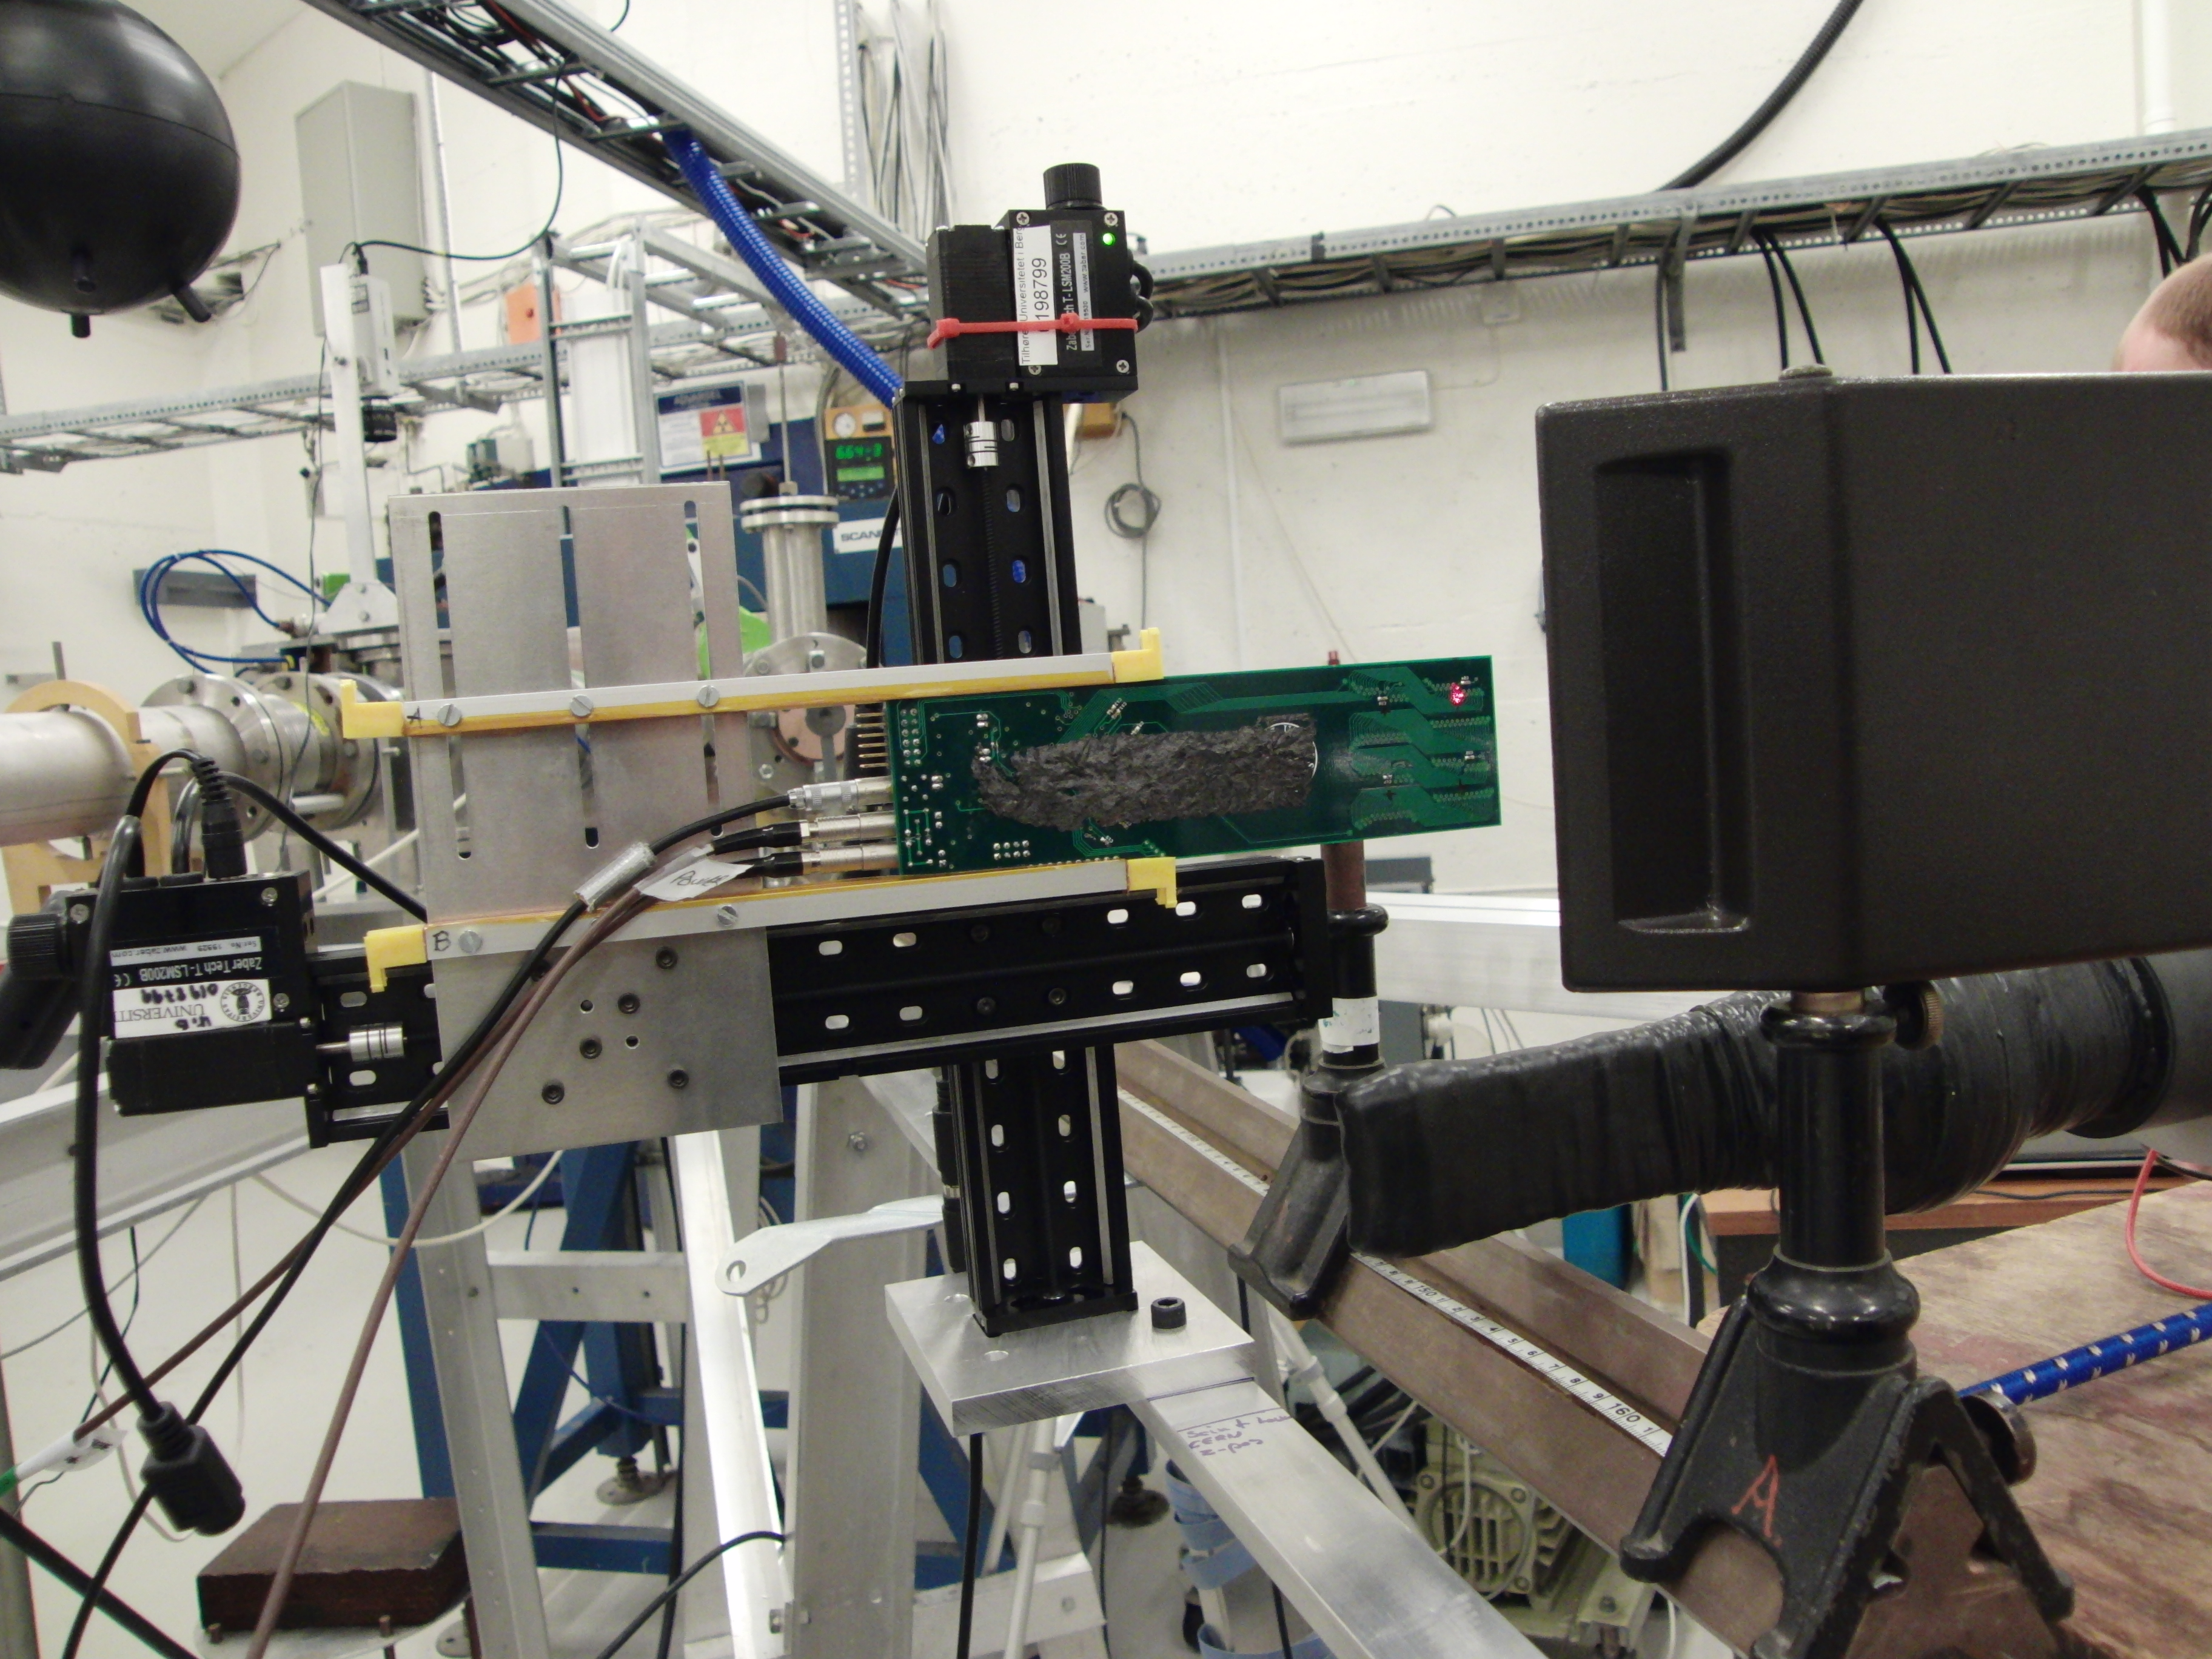
\includegraphics[width=\linewidth]{XY_back.jpg}
  \caption{SN74AVC2T245 board2}
  \end{subfigure}
 \caption{X-Y-positioning system upfront and behind, with SRAM-board mounted}
 \label{xy-table}
\end{figure}
\newpage


\chapter{Irradiation test setup}
Irradiation test for the RCU2 electronics which was discussed in the previous chapter, was executed at two facilities, that is \acf{OCL} and \acf{TSL}.
This chapter will give a brief introduction to the two facilities, and explain how we prepared ourself for test and the setup used.

\subsubsection{Purpose of tests}
The purpose of testing the RCU2 electronics for radiation is to see if the tested \ac{IC} are able to survive in a radiation hard environment as we will find in the \ac{TPC}, see section \ref{how_to_test}.
To test the limit for each of the \acp{IC}, the \acp{IC} was irradiated until a error was detected, current consumption drastically increased or the \ac{IC} received a much higher dose than was required without error.

\section{Irradiation on \ac{OCL}}
\subsection{About OCL}
Oslo cyclotron Laboratory is located at the Department of physics at the University of Oslo, and was opened in 1978. The cyclotron is of the type MC-35 and was made by Scanditronix AB from Sweden.
This is the only accelerator in Norway for ionized particles used in basic research.
The cyclotron can accelerate protons, deuteron, $^3He$ and $^4He$, 
with energies and intensities as seen in the table \ref{design requirements} bellow.
A drawing of the lab can be seen in figure \ref{OCL_fig}. 
The laboratory is divided in tree; the control room, the inner experimental hall and the outer experimental hall.
The cyclotron is placed in the inner hall, and a beam is sent through pipes to the outer hall.
There is vacuum inside the cyclotron and the pipes, so that you should not suffer energy loss from collision with air molecules.
With magnet you are able to regulate the beam to your desired pipe exit.
There are also several cups put on the pipeline which makes it possible to block the beam.
These can be used to stop the beam during an experiment, so you are able to go into the experimental area and do changes on your setup.
When the cyclotron is running and the beam is on, you are not allowed to enter the inner experimental area.
 
\begin{figure}[!htbp]
\centering
\centerline{\includegraphics[height=7cm,width=8cm]{OCL.png}}
\caption{Out-lay of the OCL}
\label{OCL_fig}
\end{figure}


\begin{table}[!htbp]
 \centering
\begin{tabular}{|l|l|l|}\hline
Ionized beam particle type & Energy(${\mega\electronvolt}$) & Intensity($\micro\ampere$)  \\ \hline \hline
Proton & 2-35 & 100 \\ \hline
Deuteron & 4-18 & 100 \\ \hline
$^3He$ &  6-47 & 50 \\ \hline 
$^4He$  & 8-35 & 50 \\ \hline
\end{tabular}
\caption{Ionized beam particle data table}
\label{design requirements}
\end{table}

\subsection{Experiment setup and equipment}

The experiment setup was placed in the outer experimental hall in experimental area 2. The experimental setup as well as the equipment used can be found in the figure and table bellow.
The equipment was kept in close to the same height around 140-150cm. Beam exit was in a height of 141.5cm.

  \vspace{5mm}
  
\begin{figure}[!htbp]
\centering
  \centerline{\includegraphics[width=0.5\textwidth]{experiment_setup.jpg}}
  \caption{Experimental setup seen from above}
  \label{experiment_setup}
\end{figure}%

  \vspace{5mm}   
  
\begin{figure}[!htbp]
  \centering
  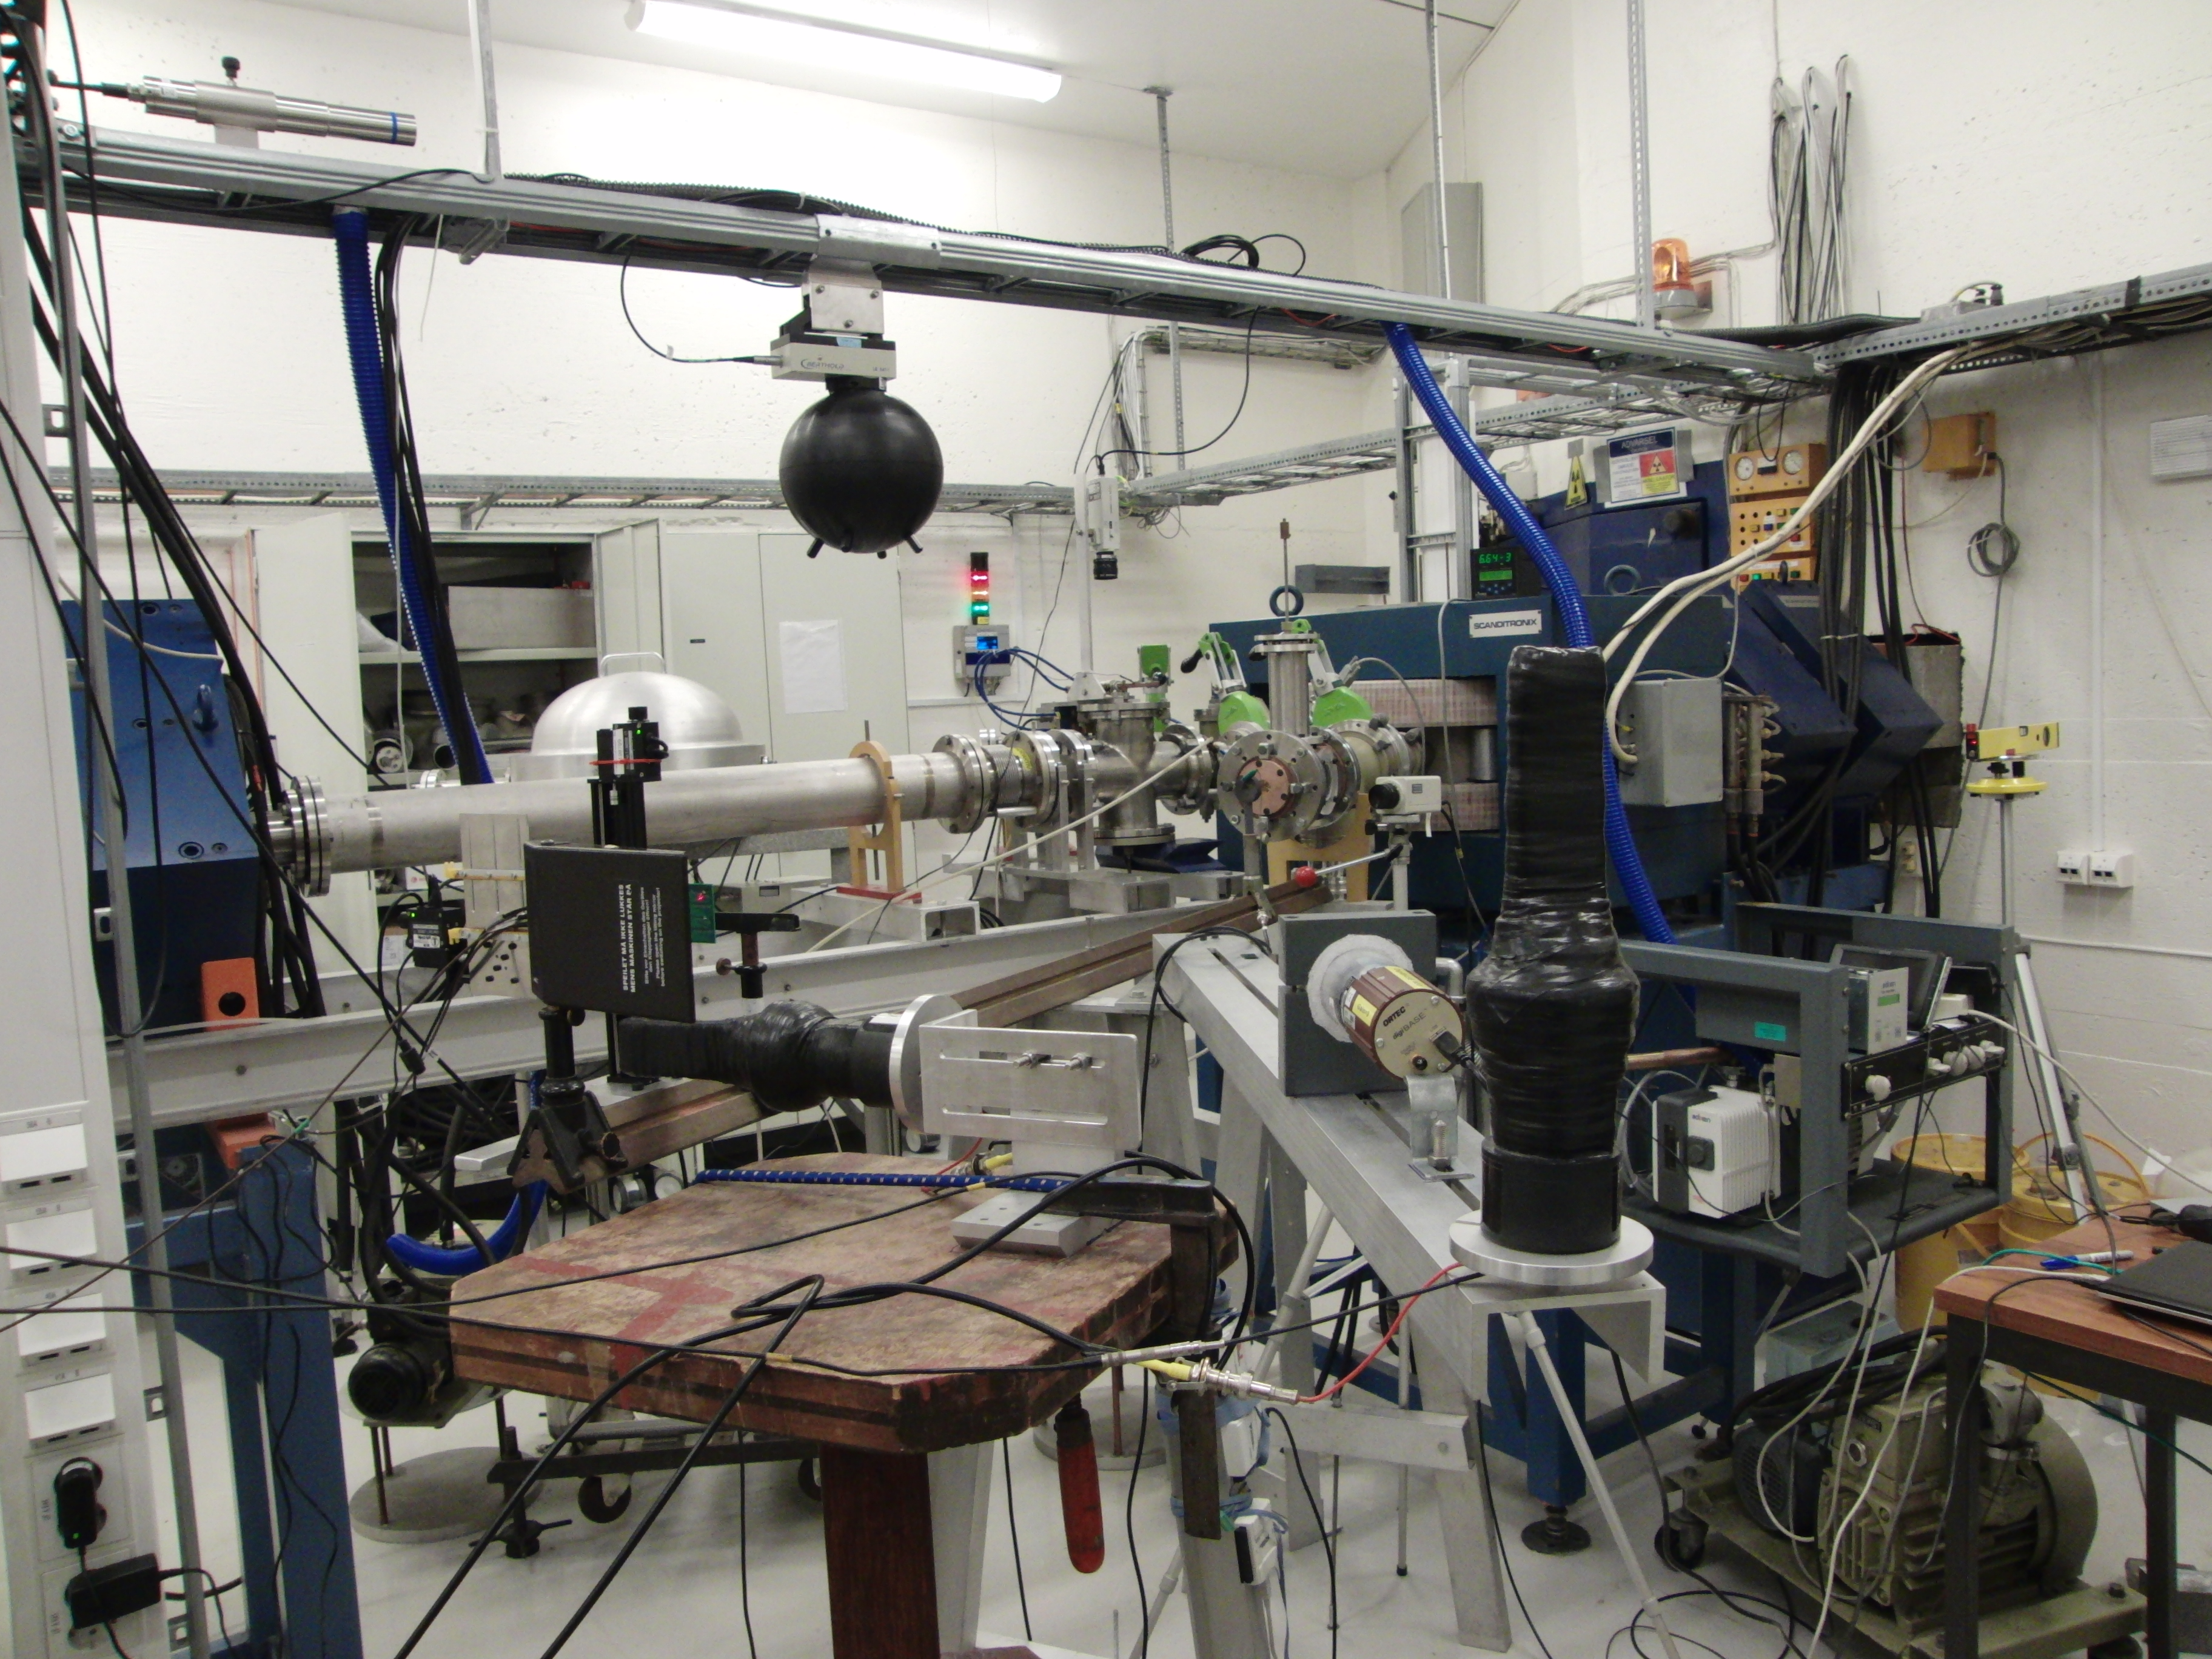
\includegraphics[width=\textwidth]{experiment_area.jpg}
  \caption{Picture of the experimental area}
  \label{experiment_area}
\end{figure}


\newpage
\begin{table}[!htbp]
 \centering
\begin{tabular}{|l|p{10cm}|}\hline
Equipment & Explanation  \\ \hline \hline
Scintillator & A plastic scintillator with photomultiplier. Was used to measure relative radiation. We had two of these, one that was placed right under \acf{DUT} and one that was placed 75cm away from \ac{DUT}. \\ \hline
High voltage regulator & Voltage for the photomultiplier. 800V was used. \\ \hline
The test boards &  TPS51200, MIC69302WU, SN74AVCB164245, SN74AVC2T245, QS3VH257, SY89831U, ADN2814, MAX3748, INA210 and TLV3011. \\ \hline 
Neutron dosimeter  & A PCB board with 4 \ac{SRAM} cells that was used to characterise the beam and to measure scintillator counts \\ \hline
SF2 starter kit & A starter kit board with the \acf{SF2} \ac{SoC} \ac{FPGA}.  \\ \hline
Computer  & A VNC server was set up on a computer inside the experimental hall, this made us able to control the experiment from the control room. The computer was running all the necessary software to control and monitor the experiment. \\ \hline
USB DAQ  & Data acquisition board form National Instruments(NI). Used to establish analog and digital connection to the test boards and send data to the computer. \\ \hline
Radiation film  & A film that reacts when irradiated. Used to identify the beam. \\ \hline
leveled laser  & Was used to pinpoint the center of the beam.\\ \hline
Mirror & Used to reflect the laser beam to the backside of the test boards.\\ \hline
XY-positioning system  & Connected to the computer so we can change the position of the test boards from a computer \\ \hline
\end{tabular}
\caption{Equipment used in the experiment}
\label{equipment}
\end{table}

\subsection{Preparation and characterization of the beam}
Before we could start testing of the \ac{PCB}, the cyclotron had to be made ready for a proton beam and the magnet controlling the direction had to be put in the right position to get the beam out in experiment area 2.



\subsubsection{Beam setup}
  \label{beam_setup}
When we were ready to start the beam test, we had to start with characterization of the beam.
The first thing to do is to get an understanding of the beam, and see that it hits around the area that we expect.
This was done by using radiation films that turns black when exposed to radiation. 
One of these was placed right in front of the beam exit and one in front of \acf{DUT} area. This was done to see how the beam spread out, and to get a feeling of where the beam center was.
A more precise calibration was done by the use of the Neutron dosimeter and the scintillator. 
By measuring the relation between scintillator counts on the scintillator which was in a locked position and SEU on the \ac{SRAM} that was connected to the XY-position system (which made the \ac{SRAM} freely to move), we were able to find a more precise position of the beam center by seeing which position gave us highest SEU counts compared to scintillator counts.
When the beam center is found and everything works as it should, the laser was placed in a position so that the laser beam points to where we had found center of the beam to be. After that we could replace the \ac{SRAM} board with the PCB that we were going to test. This had to be done every day at startup, before we could start the actual tests.

We were able to control the intensity(Current) of the beam freely from the control room inside the limitation of the beam (for protons that is up to 100 $\micro\ampere$), but we kept us in the area between 100 $\pico\ampere$ to a few $\nano\ampere$. This way the radiation dose to the test boards can be controlled. The beam intensity could be measured by putting a Faraday Cup(FC) in front of the beam. But the FC had to be removed when tests were running, since it will block the beam.

We were running 3 labVIEW programs at all time through the experiment, one for controlling the XY-position system,
one for the \ac{SRAM} board(to measure SEU and scintillator counts when calibrating and to get scintillator counts during the tests) and one program for each of the test boards.
The \ac{SRAM} and test board programs were constantly saving data on the disk.

\subsection{What was tested at OCL}
We had beam time in three periods at OCL, that is 13.11.13-15.11.13, 28.11.13-29.11.13 and 25.03.14-28.03.14.
The boards that where tested the first time are: $TPS51200_1$, $MIC69302WU_1$, $SN74AVCB164245_1$, $SN74AVC2T245_1$, $QS3VH257_1$ and $SY89831U_1$, tested in that order.
The second time, we started with the two limiting amplifier \ac{IC}, since those hadn't been tested before. So the order the \ac{PCB} was tested the second period was: $ADN2814$, $MAX3748$, $SY89831U_2$, $TPS51200_2$, $MIC69302WU_2$, $SN74AVCB164245_2$, $SN74AVC2T245_2$ and $QS3VH257_2$.
The third time at OCl, the focus was mainly the SF2 chip, but $INA210_1, INA210_2, TLV3011_1 and TLV3011_2$ was also tested.
The first time at \ac{OCL} we were given an beam of 28 MeV, but the second and third time the lab personnel manage only to produce a beam of 25 MeV.
When the beam gets out through the beam exit the energy will be reduced by crashing with air particles(~21keV per cm) \cite{}, so at DUT area the beam was respectively approx ~25 MeV and ~22 MeV.

\newpage

\section{Testing at \acf{TSL}}

\subsection{About TSL}
TSL is a national research facility located at the University of Uppsala in Sweden.
It is manly used for proton therapy by Uppsala Academic Hospital.
Beam time not used for proton therapy will be devoted to commercial neutron and proton irradiation projects. \cite{website:TSL}
TSL provides neutron and proton beams, in the range 20-180 MeV

\subsection{Beam setup procedure}


\subsection{What was tested at \ac{TSL}}

\chapter{Calculations and Results from Beam Test}
This chapter will first explain how the data collected after a radiation test was used to calculate flux and dose, followed by a presentation of the result and at the end we will have a discussion.
The result is presented after type, so that two \ac{PCB} with the same \ac{IC} are presented together.

After a radiation test on one of the PCB was done, the collected data consist of the exposed time, scintillator counts, current consumption and output data.
From the calibration before beam test, we got the relation between scintillator counts and SEU on the Neutron dosimeter. And from earlier tests the cross section for a \ac{SEU} on the Neutron dosimeter board is known.
These data is used calculate our way to the received dose for each of the different \ac{IC}. The next section will explain the calculation process.


\section{Calculation of dose}
Two ways to calculate dose will be discussed in this section, that is manually using stopping power and \ac{LET}, see section \ref{radiation_phys}, and using simulation data from a program named FLUKA. Which of these gives us the most reliable result will be discussed afterwards.

Absorbed radiation dose has the unit of energy/mass and the SI-unit is gray (Gy), which is 1 Joule of energy absorbed in a kilogram of matter[J/Kg] \ref{Joule_kg}.
Another unit which is often used when it comes to radiation of electronics is Rad, which is short for "Radiation absorbed dose".
The relation between Rad and Gy can be seen in \ref{Gy_to_Rad}.

\begin{equation}
1 Gy = 1 \frac{\joule}{\kilogram}
\label{Joule_kg}
\end{equation}

\begin{equation}
1 Rad = 100 Gy = 0.01 \frac{\joule}{\kilogram}
\label{Gy_to_Rad}
\end{equation}


\subsection{Calculating dose using LET}
When a particle enters a material, energy is deposited through ionization, and that is called \acf{LET}. To calculate the absorbed dose for a specific \ac{IC} after radiation, we have to first calculate the \ac{LET} to know the energy deposited in the \ac{IC}. But before we can do that we need to know the energy loss in air between beam exit and the test \ac{IC}. The first time at \ac{OCL} we got a 28 MeV proton beam, the two other times we only got a 25 MeV proton beam. By the use of the specific stopping power formula given in \ref{sstopping_power} we get respectively $17.516 \frac{\mega\electronvolt\centi\meter^2}{\gram}$ and $19.201 \frac{\mega\electronvolt\centi\meter^2}{\gram}$. By multiplying with the density of air which is $\rho_{air}=0.001275 \frac{\gram}{\centi\meter^3}$ we get $22.333 \frac{\mega\electronvolt}{\centi\meter}$ and $24.481 \frac{\mega\electronvolt}{\centi\meter}$. Distance between beam exit and \ac{DUT} is $130.5 \centi\meter$, which gives us:

\begin{equation}
E_{proton} = 28 - (130.5 \centi\meter \times 22.333 \frac{\mega\electronvolt}{\centi\meter}) \approx 25 \mega\electronvolt
\label{Proton_energy1}
\end{equation}

\begin{equation}
E_{proton} = 25 - (130.5 \centi\meter \times 24.481 \frac{\mega\electronvolt}{\centi\meter}) \approx 22 \mega\electronvolt
\label{Proton_energy2}
\end{equation}

Some approximations had to be done make the work easier. 

\subsection{Calculating dose using FLUKA simulations}

We start by calculating SEU from the conversion factor found in the calibration process, for 15.11.13 this was 0.0948 and for 28.11.13 this factor was 0.0473. Then we calculate the fluence at \ac{DUT} as seen in equation \ref{FluenceDUT}, and by this we can calculate the flux, see equation \ref{flux}.
To calculate the dose from here we need to know some more factors. We run a simulation on a program called FLUKA. This program is used to simulate particles in different environment. We simulated a proton beam of 28MeV and 25MeV in air, and inserted the distance from BE(Bean exit). The results can be seen in table $\ref{FLUKA_15}$.
Then we had enough information to calculate the dose. As seen from equation \ref{FluenceBE} we are able to find the Fluence at BE. And from there we can calculate the dose at \ac{DUT}, see equation \ref{DoseDUT}.


% Table generated by Excel2LaTeX from sheet 'Fluka'
\begin{table}[!htbp]
  \centering
    \begin{tabular}{|l|l|} \hline
    Fluka simulation results 28MeV &  \\\hline\hline
    Dose/primary particle at DUT[Gy] & 4,08E-10 \\\hline
    Primary particles at Beam exit & 1 \\\hline
    Primary particles at DUT & 0,1331 \\\hline
    Beam intensity reduction  at DUT & 7,513148009 \\\hline
    \end{tabular}%
      \caption{FLUKA simulation with 28MeV proton beam}
  \label{FLUKA_15}%
\end{table}%


\begin{equation}
FluenceDUT = \frac{SEU}{CS}
\label{FluenceDUT}
\end{equation}

\begin{equation}
Flux = \frac{Fluence}{time}
\label{flux}
\end{equation}

\begin{equation}
FluenceBE = \frac{fluenceDUT}{primary_particlesDUT}
\label{FluenceBE}
\end{equation}

\begin{equation}
DoseDUT[Gy] = FluenceBE \times \frac{Dose}{primary particle at DUT}
\label{DoseDUT}
\end{equation}



\section{Results from OCL}
\subsection{Calibration process}
As explained in chapter $\ref{beam_setup}$, we had to start by finding the center of the beam.
The laser was first placed in a position pointing a what thought to be center. 
Then we placed a film in front of the beam exit and \ac{DUT} area.
By seeing how the film looked like after irradiated, we got a felling of where the center was.
A example of two films from the beam exit and \ac{DUT} area can be seen in figure \ref{Radiation_film}.

\begin{figure}[!htbp]
  \centering
  \includegraphics[width=0.5\textwidth]{Radiation_film.png}
  \caption{Example of radiation films after radiation, DUT area (top) and bream exit (button). Where the laser where pointing is marked with a dot.}
  \label{Radiation_film}
\end{figure}

Now we had a feeling of where center is compared to where the laser was pointing. The Neutron dosimeter was placed with one of the SRAM chips at where the laser was pointing. This position was called position zero (x,y) = (0,0). From irradiated films, we knew approximately how much we had to move to be in center of the beam.
In table $\ref{test_15.11}$ you can see the results from our calibration 15.11.2013. You can see that position x = -2,5 cm and y = -1 cm gives highest relation between SEU and scintillator counts.
A total of 4 tests in that position was done and the average value gives us 0,0948.
When we irradiated the different \acp{PCB}, we didn't have SEU dat, but we had scintillator counts, the relation value was used to redo the scintillator count value onto \ac{SEU}. The cross section, the probability that an incoming particle will induce an SEU is known for the neutron dosimeter. The cross section (CS) is given in equation \ref{CS}. From this we could find the fluence of the beam.

% Table generated by Excel2LaTeX from sheet 'Sheet1'
\begin{table}[!htbp]
  \centering
    \begin{tabular}{|r|r|r|r|r|r|}\hline
    Calibration test nr.: & x     & y     & Scint rel & SEU(\ac{SRAM}) & SEU(\ac{SRAM})/sc \\ \hline \hline
    1     & -0,8  & -1    & 27798 & 1463  & 5,26E-02 \\ \hline
    2     & -1,3  & -1    & 17721 & 1239  & 6,99E-02 \\ \hline
    3     & -1,8  & -1    & 12904 & 1203  & 9,32E-02 \\ \hline
    4     & -2,3  & -1    & 13361 & 1276  & 9,55E-02 \\ \hline
    5     & -2,8  & -1    & 12786 & 1238  & 9,68E-02 \\ \hline
    6     & -3,3  & -1    & 12342 & 1156  & 9,37E-02 \\ \hline
    7     & -2,5  & -1    & 11696 & 1223  & 1,05E-01 \\ \hline
    8     & -2,5  & -1,5  & 11027 & 1075  & 9,75E-02 \\ \hline
    9     & -2,5  & -2    & 11835 & 1063  & 8,98E-02 \\ \hline
    10    & -2,5  & -0,5  & 15593 & 1540  & 9,88E-02 \\ \hline
    11    & -2,5  & 0     & 12620 & 1034  & 8,19E-02 \\ \hline
    12    & -2,5  & -1    & 65280 & 5999  & 9,19E-02 \\ \hline
    13    & -2,5  & -1    & 52752 & 4803  & 9,10E-02 \\ \hline
    14    & -2,5  & -1    & 57229 & 5250  & 9,17E-02 \\ \hline
    \end{tabular}%
      \caption{Calibration tests 15.11.2013}
  \label{test_15.11}%
\end{table}%

\begin{equation}
CS = 1,14e-6
\label{CS}
\end{equation}

\section{Test results}
The tests was controlled and monitored through a LabVIEW program for each of the different IC. When testing ADN2814 and MAX3748 there was also needed a \ac{SF2} board to produce a input signal, and compare the input with the output signal. A complete result of the tests can be found in appendix \ref{appendix}.
The point of this test was to see that these ICs would survive in a radiated area. The total dose of 10 years in the ALICE detector is estimated to be a 1-2 kRad, see section \ref{how_to_test}. If a \ac{IC} survives more than 10 times that, we can be quite sure that it will survive the radiation it will receive at CERN.
In table \ref{dose_15.11} and \ref{dose_28.11} you can see how long each ICs has been exposed too radiation, the dose they have been received and if an error occurred.

\begin{table}[!htbp]
 \centering
\begin{tabular}{|l|l|l|l|}\hline
Device & Exposed time[s] & Dose[Rad] & Error \\ \hline \hline
$TPS51200$ & 2065 & 41800 & No \\ \hline
$MIC69302WU_1$ & 2240 & 164000 & No \\ \hline
$SN74AVCB164245_1$ & 967  & 65200 & No \\ \hline
$SN74AVC2T245_1$ & 860  & 4600 & Yes \\ \hline
$QS3VH257_1$ & 795  & 52800 & No \\ \hline
$SY89831_1$ & 1251 & 93500 & No \\ \hline
\end{tabular}
\caption{Tests at OCL 15.nov 2013}
\label{dose_15.11}
\end{table}

\begin{table}[!htbp]
 \centering
\begin{tabular}{|l|l|l|l|}\hline
Device & Exposed time[s] & Dose[Rad] &  \\ \hline \hline
$ADN2814/_run1$ & 1273 & 20200 & Yes \\ \hline
$ADN2814/_run2$ & 2286 & 324900 & Yes \\ \hline
$MAX3748$ & 2384 & 442200 & No \\ \hline
$TPS51200_2$ & -\textsuperscript{*} & -* & -* \\ \hline
$MIC69302WU_2$ & 1385 & 383800 & No \\ \hline
$SN74AVCB164245_2$ & 526  & 201400 & No \\ \hline
$SN74AVC2T245_2$ & 478  & 161600 & No \\ \hline
$QS3VH257_2$ & 264  & 110300 & No \\ \hline
$SY89831U_2$ & 921  & 165800 & No \\ \hline
\multicolumn{4}{l}{\textsuperscript{*}\footnotesize{The board wouldn't work at test time}}
\end{tabular}
\caption{Tests at OCL 27-28.nov 2013}
\label{dose_28.11}
\end{table}

\begin{figure}[!htbp]
  \centering
  \includegraphics[width=\textwidth]{flux_all_test1.jpg}
  \caption{flux for each component radiated 15.11.2013}
  \label{flux_all1}
\end{figure}

\begin{figure}[!htbp]
  \centering
  \includegraphics[width=\textwidth]{Flux_vs_time_all.jpg}
  \caption{flux for each component radiated 15.11.2013}
  \label{flux_all2}
\end{figure}
\newpage
In figure $\ref{flux_all1}$ and $\ref{flux_all2}$ you can see graphs of flux vs time for the different test boards. The reason the graphs don't go as linear as one would expect, is that the beam sometimes stopped and had to restarted, and that we increased and decreased the intensities as we wanted.

\FloatBarrier

\subsection{TPS51200}
This was the first board that was tested.
The intensity was a little low on this test.
To make the testing process faster the intensity was increased during the later experiments.

The IC worked after a dose of 40kRad, but we could see a little increase in current after a dose of 25 kRad. The output voltage is close to stable, a few mV up and down, but not noteworthy.
Two PCBs of this type was tested, but only one worked when we was at OCL to do the testing.

\begin{figure}[!htbp]
\centering
  \includegraphics[width=.49\textwidth]{current_voltage_tps.jpg}
  \caption{TPS51200 - Current/Voltage vs Dose}
  \label{TPS51200_1}
\end{figure}

\FloatBarrier

\subsection{MIC69302WU}
The first board was tested 15.11.13 and the second board was tested 28.11.13. During the test of the first board we increased the intensity of the beam quite allot, that can be seen from the flux graph, in figure \ref{flux_all1}.

This \ac{IC} had an unexpected reaction to irradiation. You can see from both of the graphs that the current is decreasing and voltage is increasing, normally we would expect the opposite, or at least that the current would increase.
As seen from the graph in figure \ref{MIC69302WU_both} it starts quite early to decrease in current, but as you can see it also stabilize after a while. The output voltage is mostly stable, there were a increase of ~2\% on both of the tests.

\begin{figure}[!htbp]
\centering
  \begin{subfigure}{.49\textwidth}
  \centering
  \includegraphics[width=\linewidth]{current_voltage_mic.jpg}
  \caption{MIC69302WU board1}
  \label{MIC69302WU_1}
  \end{subfigure}
  \begin{subfigure}{.49\textwidth}
  \centering
  \includegraphics[width=\linewidth]{current_volt_dose_MIC.jpg}
  \caption{MIC69302WU board2}
  \label{MIC69302WU_2}
  \end{subfigure}
 \caption{MIC69302WU - Current/Voltage vs Dose}
 \label{MIC69302WU_both}
\end{figure}

\FloatBarrier

\subsection{SN74AVCB164245}

It can be seen that the characteristics on the two test board are different, the reason for this is maybe because of different output load. The reason for the ``jumps`` in current is because the output is constantly changing from on to off, with a gap of 4 seconds.
This chips is not effected by radiation before a dose of approx 40kRad. That is more than enough for the purposes we are going to use this for.

\begin{figure}[!htbp]
\centering
  \begin{subfigure}{.49\textwidth}
  \centering
  \includegraphics[width=\linewidth]{current_4245.jpg}
  \caption{SN74AVCB164245 board1}
  \label{SN74AVCB164245_1}
  \end{subfigure}
  \begin{subfigure}{.49\textwidth}
  \centering
  \includegraphics[width=\linewidth]{current_dose_42452.jpg}
  \caption{SN74AVCB164245 board2}
  \label{SN74AVCB164245_2}
  \end{subfigure}
 \caption{SN74AVC2T245 - Current vs Dose}
\end{figure}

\FloatBarrier

\subsection{SN74AVC2T245}

Something went wrong on the first test. After 740 s and a dose of 98 Rad the chips output was stuck at 1. The reason for this is unknown, I fear that this might be defected before we started the test, since it gives a totally different characteristics than test board nr 2.
The input was switching from high to low every 4 second. If we look at the test results from board 2, the current goes unchanged up to 40 kRad, and that is more than enough.
%her m� eg sjekke board1 etter eg har f�tt den tilbake, og se om den faktisk fungere. Kan hende at denne har v�rt �delagt f�r vi begynte.

\begin{figure}[!htbp]
\centering
  \begin{subfigure}{.49\textwidth}
  \centering
  \includegraphics[width=\linewidth]{current_t245.jpg}
  \caption{SN74AVC2T245 board1}
  \label{SN74AVC2T245_1}
  \end{subfigure}
  \begin{subfigure}{.49\textwidth}
  \centering
  \includegraphics[width=\linewidth]{current_dose_t2452.jpg}
  \caption{SN74AVC2T245 board2}
  \label{SN74AVC2T245_2}
  \end{subfigure}
 \caption{SN74AVC2T245 - Current vs Dose}
\end{figure}

\FloatBarrier

\subsection{QS3VH257}
The select input was changed every 4 second and the inputs(I0A, I0B, I0C, I0D, I1A, I1B, I1C and I1D) was inverted every 18 second.

The two test boards worked fine through the tests.
We see that we have small increase in current before 30 kRad, after that it increases quite allot. We couldn't see any errors on the output during the experiment, but it should probably not be exposed to more than 30 kRad.

\begin{figure}[!htbp]
\centering
  \begin{subfigure}{.49\textwidth}
  \centering
  \includegraphics[width=\linewidth]{current_q.jpg}
  \caption{QS3VH257 board1}
  \label{QS3VH257_1}
  \end{subfigure}
  \begin{subfigure}{.49\textwidth}
  \centering
  \includegraphics[width=\linewidth]{current_dose_q2.jpg}
  \caption{QS3VH257 board2}
  \label{QS3VH257_2}
  \end{subfigure}
 \caption{QS3VH257 - Current vs Dose}
\end{figure}

\FloatBarrier

\subsection{SY89831}
This \ac{IC} required a high current to work, and since the labVIEW DAQ device only delivers 5mA on the analog outputs, a combination of the modified MIC69302WU as described in section \ref{MIC_explanation} and the 5V output on the DAQ was used. This gave us a output of 3.3 V and a current limit of 200 mA. Here a 20$\ohm$ resistor was used to measure current instead of a 220 $\ohm$ resistor, this was to reduce the voltage drop over the resistor because of the high current consumption.

A difference in characteristics can also be seen here. This may be because two different footprint for the PCB was used, and therefore some difference can be seen. We see a small increase in current on both of the boards, but not noteworthy, compared to how much current this IC is using.


\begin{figure}[!htbp]
\centering
  \begin{subfigure}{.49\textwidth}
  \centering
  \includegraphics[width=\linewidth]{current_sy.jpg}
  \caption{SY89831 board1}
  \label{SY89831_1}
  \end{subfigure}
  \begin{subfigure}{.49\textwidth}
  \centering
  \includegraphics[width=\linewidth]{current_dose_SY2.jpg}
  \caption{SY89831 board2}
  \label{SY89831_2}
  \end{subfigure}
 \caption{SY89831 - Current vs Dose}
\end{figure}

\FloatBarrier

\subsection{ADN2814}
This \ac{IC} is a little special and was hard to get a good test on. This is a clock and data return circuit, with a limiting amplifier.
The SF2 board was used to code a clock and data into a differential Manchester signal, that was sent into the IC. Out of the IC we get a LVDS clock and LVDS Manchester signal. The Manchester coded data signal was decoded on SF2 board, so that we get out a clock and data. The data was tested by delaying the original data through a few D-latches, so that the original and returned data was close to synced. Then we could compare the original data with the one from the \ac{IC} through a XOR-function. This function was triggered by a 80 Mhz clock from the \ac{SF2} board. If they aren't equal when the clock rises, a 1 will be added to a counter. The value of the counter was constantly sent through the UART of the SF2 board.

The way the clock was tested was a little harder process since the clock was so fast (160 Mhz).
This was solved, was by adding a third clock with the same frequency (160 Mhz) that was $90\,^{\circ}$ of from the two others, when this goes high I called on the XOR-function, to see if the two other clocks are the same. if they are alike, nothing happens, if they are not the program adds 1 to a counter, which constantly writes its current value to a \acf{UART}.
The problem here is that for each time the \ac{SF2} board was programed the clock was slightly different, that made either the clock out of sync or the data out of sync, so the code didn't always work as it should.
This circuit also requires allot of current, therefore the same solution as for SY89831 was used, using MIC69302WU as a power supply and measure the current on that PCB.

The current didn't change before a dose of 200 kRad had been received, but we got a clock error at a dose of $ \sim $11 kRad, and a data error after a dose of $ \sim $8 kRad.
How good this test really is, could be discussed, since we don't have any data on the clock and data, other than that the XOR-function failed. What really failed, and how much is impossible to know. It could be a slightly delay on a clock or the data, or maybe the clock just disappeared for a moment.

\begin{figure}[!htbp]
\centering
  \begin{subfigure}{.49\textwidth}
  \centering
  \includegraphics[width=\linewidth]{current_dose_ADN_t1.jpg}
  \caption{ADN2814 test1}
  \label{ADN2814_1}
  \end{subfigure}
  \begin{subfigure}{.49\textwidth}
  \centering
  \includegraphics[width=\linewidth]{current_dose_ADN_t2.jpg}
  \caption{ADN2814 test2}
  \label{ADN2814_2}
  \end{subfigure}
 \caption{ADN2814 - Current vs Dose}
\end{figure}

\begin{figure}[!htbp]
\centering
  \begin{subfigure}{.49\textwidth}
  \centering
  \includegraphics[width=\linewidth]{error_dose_ADN_t1.jpg}
  \caption{ADN2814 test1}
  \label{ADN2814_1e}
  \end{subfigure}
  \begin{subfigure}{.49\textwidth}
  \centering
  \includegraphics[width=\linewidth]{error_dose_ADN_t2.jpg}
  \caption{ADN2814 test2}
  \label{ADN2814_2e}
  \end{subfigure}
 \caption{ADN2814 - Relative errors vs Dose}
\end{figure}

\FloatBarrier

\subsection{MAX3748}
This circuit has the same purpose as ADN2814, the difference is that this one only return the limited Manchester coded signal, and no clock. The process for testing the data is the same as for the ADN2814.
The decoding process return clock and data, but since they are related to another, a error on the clock would mean an error at the data. So by measuring data, we can be sure that there are no clock errors as well. 

After a dose of over 400 kRad this chip still worked, and current consumption was stable through the hole irradiation process.

\begin{figure}[!htbp]
\centering
  \begin{subfigure}{.49\textwidth}
  \centering
  \includegraphics[width=\linewidth]{current_dose_MAX.jpg}
  \caption{Current vs Dose}
  \label{MAX3748}
  \end{subfigure}
  \begin{subfigure}{.49\textwidth}
  \centering
  \includegraphics[width=\linewidth]{error_dose_MAX.jpg}
  \caption{Errors vs Dose}
  \label{MAX3748_error}
  \end{subfigure}
 \caption{MAX3748}
\end{figure}

\FloatBarrier


\newpage
\section{Discussion of the result}
Most of the testing was done 15.nov and 28.nov. The other days was used to get familiar with the instruments and equipment that was being used, to prepare the setup and setting up the beam.
There are almost impossible to get the same beam two days at a row. Each day of testing is therefore different from each other. Since the testing was conducted in two periodes and a total of 4 test days, there are allot of uncertainties regarding the beam.
And that is also why we had to do calibration each day at start-up.

When we were going to measure the intensity at the beam exit, we placed a Faraday cup in front of the beam, and connected it to a amperemeter on the control panel, but since the current is so small, the measuring instrument will be affected by air currents, and there are also allot of uncertainties in the instruments. Therefore we only used the Faraday cup and the amperemeter, to get a rough estimate of the actual intensity.

The are also some uncertainties regarding the DAQ device form NI. When measuring digital signal, we don't know if it goes from 0 V to 3.3 V as we would expect. Maybe in reality the low voltage is actually 0.4 V and high voltage is actually 2.8 V. If this is the case, it could be a problem with using this in our design.

As said before in \ref{beam_setup}, if a component survives 10 times more than what it will receive in a period of 10 years in ALICE, that is 1-2 kRad, than it can be used in the design of RCU2.
Having that in mind, I would say that every component tested would have a green flag even though we had some errors when testing SN74AVC2T245 and ADN2814. Since the result after testing board two of SN74AVC2T245 was positive we can assume that something was wrong with the first board. When it comes to ADN2814, it would be nice to have more time in the lab to test this even more, since the test done gave us so unclear results. If a better test would be made, I'm sure that this would perform much better.

\newpage

\chapter{Conclusion}



\FloatBarrier

\begin{appendices}
\chapter{Some Appendix}
\label{appendix}

\section{datasheets}
\label{datasheets}
% Table generated by Excel2LaTeX from sheet 'Sheet1'
\begin{table}
  \centering
    \begin{tabular}{|l|l|l|l|l|l|} \hline
    Calibration test nr.: & x     & y     & Scint rel & SEU(\ac{SRAM}) & SEU(\ac{SRAM})/sc \\ \hline \hline
    1     & 0     & 0     & 23813 & 1971  & 8,28E-02 \\ \hline
    2     & 0     & -0,5  & 37930 & 3867  & 1,02E-01 \\ \hline
    3     & 0     & -1    & 27527 & 2817  & 1,02E-01 \\ \hline
    4     & 0     & -1,5  & 34413 & 3360  & 9,76E-02 \\ \hline
    5     & 0     & -2    & 32713 & 2763  & 8,45E-02 \\ \hline
    6     & 0,5   & 0     & 38753 & 2709  & 6,99E-02 \\ \hline
    7     & -0,5  & 0     & 23420 & 2483  & 1,06E-01 \\ \hline
    8     & -1    & 0     & 20611 & 2232  & 1,08E-01 \\ \hline	
    9     & -1,5  & 0     & 21014 & 2410  & 1,15E-01 \\ \hline
    10    & -1,5  & 0     & 20676 & 2260  & 1,09E-01 \\ \hline
    11    & -2    & 0     & 35787 & 3776  & 1,06E-01 \\ \hline
    12    & -2,5  & 0     & 27847 & 2512  & 9,02E-02 \\ \hline
    \end{tabular}%
      \caption{Calibration tests 14.11.2013}
      \label{test_14.11}
\end{table}%

% Table generated by Excel2LaTeX from sheet 'Sheet1'
\begin{table}
  \centering
    \begin{tabular}{|l|l|l|l|l|l|}\hline
    Calibration test nr.: & x     & y     & Scint rel & SEU(\ac{SRAM}) & SEU(\ac{SRAM})/ sc \\ \hline \hline
    1     & -0,8  & -1    & 27798 & 1463  & 5,26E-02 \\ \hline
    2     & -1,3  & -1    & 17721 & 1239  & 6,99E-02 \\ \hline
    3     & -1,8  & -1    & 12904 & 1203  & 9,32E-02 \\ \hline
    4     & -2,3  & -1    & 13361 & 1276  & 9,55E-02 \\ \hline
    5     & -2,8  & -1    & 12786 & 1238  & 9,68E-02 \\ \hline
    6     & -3,3  & -1    & 12342 & 1156  & 9,37E-02 \\ \hline
    7     & -2,5  & -1    & 11696 & 1223  & 1,05E-01 \\ \hline
    8     & -2,5  & -1,5  & 11027 & 1075  & 9,75E-02 \\ \hline
    9     & -2,5  & -2    & 11835 & 1063  & 8,98E-02 \\ \hline
    10    & -2,5  & -0,5  & 15593 & 1540  & 9,88E-02 \\ \hline
    11    & -2,5  & 0     & 12620 & 1034  & 8,19E-02 \\ \hline
    12    & -2,5  & -1    & 65280 & 5999  & 9,19E-02 \\ \hline
    13    & -2,5  & -1    & 52752 & 4803  & 9,10E-02 \\ \hline
    14    & -2,5  & -1    & 57229 & 5250  & 9,17E-02 \\ \hline
    \end{tabular}%
      \caption{Calibration tests 15.11.2013}
\end{table}%

% Table generated by Excel2LaTeX from sheet 'Fluka'
\begin{table}
  \centering
    \begin{tabular}{|l|l|} \hline
    Fluka simulation results 28MeV &  \\\hline\hline
    Dose/primary particle at DUT[Gy] & 4,08E-10 \\\hline
    Primary particles at Beam exit & 1 \\\hline
    Primary particles at DUT & 0,1331 \\\hline
    Beam intensity reduction  at DUT & 7,513148009 \\\hline
    \end{tabular}%
      \caption{FLUKA simulation with 28MeV proton beam}
\end{table}%

% Table generated by Excel2LaTeX from sheet 'Fluka'
\begin{table}
  \centering
    \begin{tabular}{|l|l|}\hline
    Fluka simulation results 25MeV &  \\\hline\hline
    $\frac{Dose}{primary particle at DUT}$[Gy] & 2,94E-10 \\\hline
    Primary particles at Beam exit & 1 \\\hline
    Primary particles at DUT & 8,57E-02 \\\hline
    Beam intensity reduction  at DUT & 11,6713352 \\\hline
    \end{tabular}%
    \caption{FLUKA simulation with 25MeV proton beam}
  \label{FLUKA_28}%
\end{table}%

\end{appendices}

\FloatBarrier

\newpage
\bibliographystyle{plain}
\bibliography{Master_Thesis_Inge_Nikolai_Torsvik}
\end{document}